\documentclass[1p]{elsarticle_modified}
%\bibliographystyle{elsarticle-num}

%\usepackage[colorlinks]{hyperref}
%\usepackage{abbrmath_seonhwa} %\Abb, \Ascr, \Acal ,\Abf, \Afrak
\usepackage{amsfonts}
\usepackage{amssymb}
\usepackage{amsmath}
\usepackage{amsthm}
\usepackage{scalefnt}
\usepackage{amsbsy}
\usepackage{kotex}
\usepackage{caption}
\usepackage{subfig}
\usepackage{color}
\usepackage{graphicx}
\usepackage{xcolor} %% white, black, red, green, blue, cyan, magenta, yellow
\usepackage{float}
\usepackage{setspace}
\usepackage{hyperref}

\usepackage{tikz}
\usetikzlibrary{arrows}

\usepackage{multirow}
\usepackage{array} % fixed length table
\usepackage{hhline}

%%%%%%%%%%%%%%%%%%%%%
\makeatletter
\renewcommand*\env@matrix[1][\arraystretch]{%
	\edef\arraystretch{#1}%
	\hskip -\arraycolsep
	\let\@ifnextchar\new@ifnextchar
	\array{*\c@MaxMatrixCols c}}
\makeatother %https://tex.stackexchange.com/questions/14071/how-can-i-increase-the-line-spacing-in-a-matrix
%%%%%%%%%%%%%%%

\usepackage[normalem]{ulem}

\newcommand{\msout}[1]{\ifmmode\text{\sout{\ensuremath{#1}}}\else\sout{#1}\fi}
%SOURCE: \msout is \stkout macro in https://tex.stackexchange.com/questions/20609/strikeout-in-math-mode

\newcommand{\cancel}[1]{
	\ifmmode
	{\color{red}\msout{#1}}
	\else
	{\color{red}\sout{#1}}
	\fi
}

\newcommand{\add}[1]{
	{\color{blue}\uwave{#1}}
}

\newcommand{\replace}[2]{
	\ifmmode
	{\color{red}\msout{#1}}{\color{blue}\uwave{#2}}
	\else
	{\color{red}\sout{#1}}{\color{blue}\uwave{#2}}
	\fi
}

\newcommand{\Sol}{\mathcal{S}} %segment
\newcommand{\D}{D} %diagram
\newcommand{\A}{\mathcal{A}} %arc


%%%%%%%%%%%%%%%%%%%%%%%%%%%%%5 test

\def\sl{\operatorname{\textup{SL}}(2,\Cbb)}
\def\psl{\operatorname{\textup{PSL}}(2,\Cbb)}
\def\quan{\mkern 1mu \triangleright \mkern 1mu}

\theoremstyle{definition}
\newtheorem{thm}{Theorem}[section]
\newtheorem{prop}[thm]{Proposition}
\newtheorem{lem}[thm]{Lemma}
\newtheorem{ques}[thm]{Question}
\newtheorem{cor}[thm]{Corollary}
\newtheorem{defn}[thm]{Definition}
\newtheorem{exam}[thm]{Example}
\newtheorem{rmk}[thm]{Remark}
\newtheorem{alg}[thm]{Algorithm}

\newcommand{\I}{\sqrt{-1}}
\begin{document}

%\begin{frontmatter}
%
%\title{Boundary parabolic representations of knots up to 8 crossings}
%
%%% Group authors per affiliation:
%\author{Yunhi Cho} 
%\address{Department of Mathematics, University of Seoul, Seoul, Korea}
%\ead{yhcho@uos.ac.kr}
%
%
%\author{Seonhwa Kim} %\fnref{s_kim}}
%\address{Center for Geometry and Physics, Institute for Basic Science, Pohang, 37673, Korea}
%\ead{ryeona17@ibs.re.kr}
%
%\author{Hyuk Kim}
%\address{Department of Mathematical Sciences, Seoul National University, Seoul 08826, Korea}
%\ead{hyukkim@snu.ac.kr}
%
%\author{Seokbeom Yoon}
%\address{Department of Mathematical Sciences, Seoul National University, Seoul, 08826,  Korea}
%\ead{sbyoon15@snu.ac.kr}
%
%\begin{abstract}
%We find all boundary parabolic representation of knots up to 8 crossings.
%
%\end{abstract}
%\begin{keyword}
%    \MSC[2010] 57M25 
%\end{keyword}
%
%\end{frontmatter}

%\linenumbers
%\tableofcontents
%
\newcommand\colored[1]{\textcolor{white}{\rule[-0.35ex]{0.8em}{1.4ex}}\kern-0.8em\color{red} #1}%
%\newcommand\colored[1]{\textcolor{white}{ #1}\kern-2.17ex	\textcolor{white}{ #1}\kern-1.81ex	\textcolor{white}{ #1}\kern-2.15ex\color{red}#1	}

{\Large $\underline{12n_{0556}~(K12n_{0556})}$}

\setlength{\tabcolsep}{10pt}
\renewcommand{\arraystretch}{1.6}
\vspace{1cm}\begin{tabular}{m{100pt}>{\centering\arraybackslash}m{274pt}}
\multirow{5}{120pt}{
	\centering
	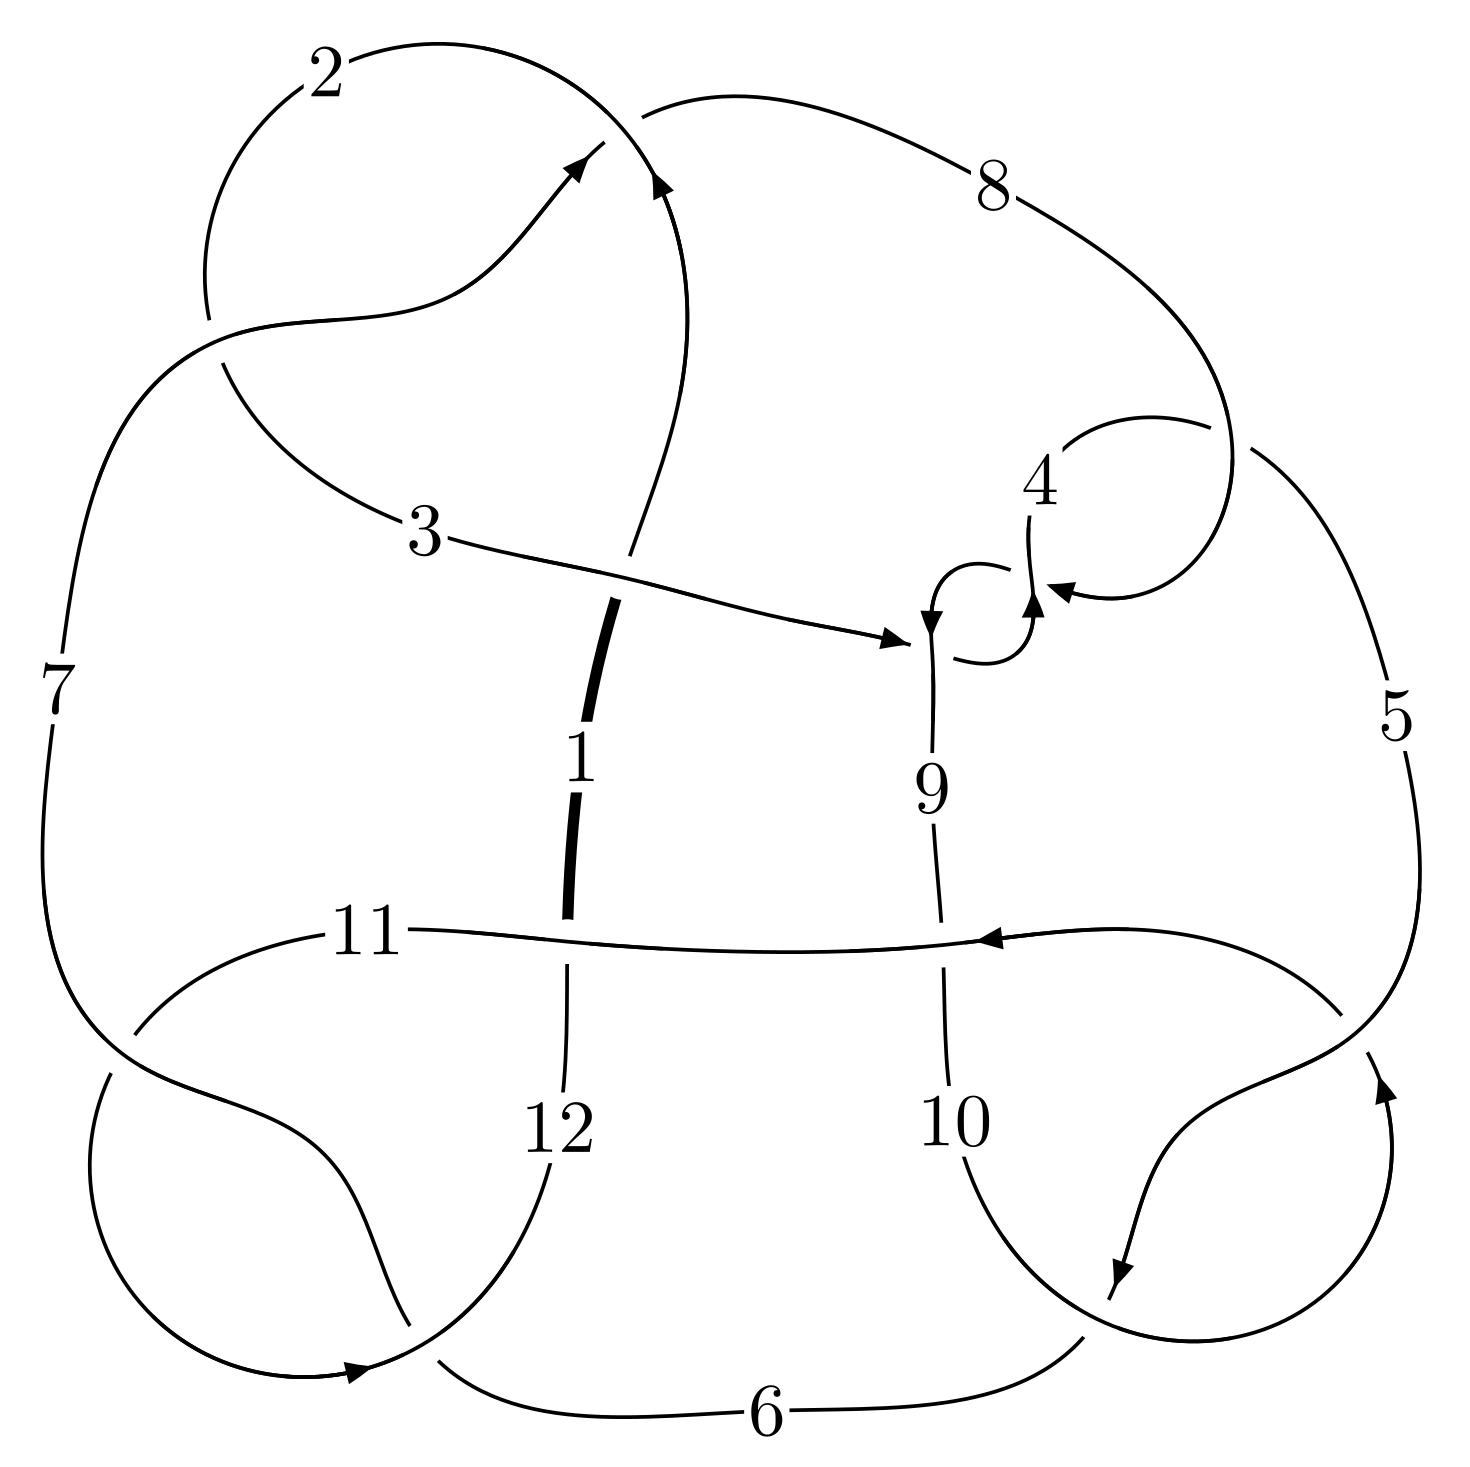
\includegraphics[width=112pt]{../../../GIT/diagram.site/Diagrams/png/2645_12n_0556.png}\\
\ \ \ A knot diagram\footnotemark}&
\allowdisplaybreaks
\textbf{Linearized knot diagam} \\
\cline{2-2}
 &
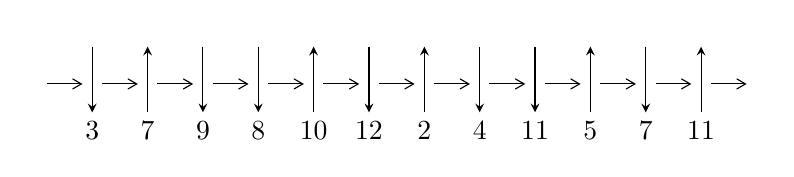
\begin{tikzpicture}[x=20pt, y=17pt]
	% nodes
	\node (C0) at (0, 0) {};
	\node (C1) at (1, 0) {};
	\node (C1U) at (1, +1) {};
	\node (C1D) at (1, -1) {3};

	\node (C2) at (2, 0) {};
	\node (C2U) at (2, +1) {};
	\node (C2D) at (2, -1) {7};

	\node (C3) at (3, 0) {};
	\node (C3U) at (3, +1) {};
	\node (C3D) at (3, -1) {9};

	\node (C4) at (4, 0) {};
	\node (C4U) at (4, +1) {};
	\node (C4D) at (4, -1) {8};

	\node (C5) at (5, 0) {};
	\node (C5U) at (5, +1) {};
	\node (C5D) at (5, -1) {10};

	\node (C6) at (6, 0) {};
	\node (C6U) at (6, +1) {};
	\node (C6D) at (6, -1) {12};

	\node (C7) at (7, 0) {};
	\node (C7U) at (7, +1) {};
	\node (C7D) at (7, -1) {2};

	\node (C8) at (8, 0) {};
	\node (C8U) at (8, +1) {};
	\node (C8D) at (8, -1) {4};

	\node (C9) at (9, 0) {};
	\node (C9U) at (9, +1) {};
	\node (C9D) at (9, -1) {11};

	\node (C10) at (10, 0) {};
	\node (C10U) at (10, +1) {};
	\node (C10D) at (10, -1) {5};

	\node (C11) at (11, 0) {};
	\node (C11U) at (11, +1) {};
	\node (C11D) at (11, -1) {7};

	\node (C12) at (12, 0) {};
	\node (C12U) at (12, +1) {};
	\node (C12D) at (12, -1) {11};
	\node (C13) at (13, 0) {};

	% arrows
	\draw[->,>={angle 60}]
	(C0) edge (C1) (C1) edge (C2) (C2) edge (C3) (C3) edge (C4) (C4) edge (C5) (C5) edge (C6) (C6) edge (C7) (C7) edge (C8) (C8) edge (C9) (C9) edge (C10) (C10) edge (C11) (C11) edge (C12) (C12) edge (C13) ;	\draw[->,>=stealth]
	(C1U) edge (C1D) (C2D) edge (C2U) (C3U) edge (C3D) (C4U) edge (C4D) (C5D) edge (C5U) (C6U) edge (C6D) (C7D) edge (C7U) (C8U) edge (C8D) (C9U) edge (C9D) (C10D) edge (C10U) (C11U) edge (C11D) (C12D) edge (C12U) ;
	\end{tikzpicture} \\
\hhline{~~} \\& 
\textbf{Solving Sequence} \\ \cline{2-2} 
 &
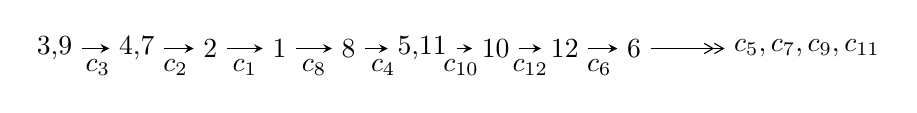
\begin{tikzpicture}[x=25pt, y=7pt]
	% node
	\node (A0) at (-1/8, 0) {3,9};
	\node (A1) at (17/16, 0) {4,7};
	\node (A2) at (17/8, 0) {2};
	\node (A3) at (25/8, 0) {1};
	\node (A4) at (33/8, 0) {8};
	\node (A5) at (83/16, 0) {5,11};
	\node (A6) at (25/4, 0) {10};
	\node (A7) at (29/4, 0) {12};
	\node (A8) at (33/4, 0) {6};
	\node (C1) at (1/2, -1) {$c_{3}$};
	\node (C2) at (13/8, -1) {$c_{2}$};
	\node (C3) at (21/8, -1) {$c_{1}$};
	\node (C4) at (29/8, -1) {$c_{8}$};
	\node (C5) at (37/8, -1) {$c_{4}$};
	\node (C6) at (23/4, -1) {$c_{10}$};
	\node (C7) at (27/4, -1) {$c_{12}$};
	\node (C8) at (31/4, -1) {$c_{6}$};
	\node (A9) at (43/4, 0) {$c_{5},c_{7},c_{9},c_{11}$};

	% edge
	\draw[->,>=stealth]	
	(A0) edge (A1) (A1) edge (A2) (A2) edge (A3) (A3) edge (A4) (A4) edge (A5) (A5) edge (A6) (A6) edge (A7) (A7) edge (A8) ;
	\draw[->>,>={angle 60}]	
	(A8) edge (A9);
\end{tikzpicture} \\ 

\end{tabular} \\

\footnotetext{
The image of knot diagram is generated by the software ``\textbf{Draw programme}" developed by Andrew Bartholomew(\url{http://www.layer8.co.uk/maths/draw/index.htm\#Running-draw}), where we modified some parts for our purpose(\url{https://github.com/CATsTAILs/LinksPainter}).
}\phantom \\ \newline 
\centering \textbf{Ideals for irreducible components\footnotemark of $X_{\text{par}}$} 
 
\begin{align*}
I^u_{1}&=\langle 
u^7+u^6+2 u^5+3 u^4-2 u^3+6 u^2+4 d- u+2,\;- u^7- u^6-4 u^5+u^4-2 u^3+8 u^2+4 c- u,\\
\phantom{I^u_{1}}&\phantom{= \langle  }- u^7+u^6-6 u^5+5 u^4-12 u^3+8 u^2+4 b-5 u+2,\;u^7- u^6+4 u^5-5 u^4+4 u^3-6 u^2+4 a- u,\\
\phantom{I^u_{1}}&\phantom{= \langle  }u^8+5 u^6-3 u^5+7 u^4-8 u^3+5 u^2- u+2\rangle \\
I^u_{2}&=\langle 
u^5- u^4+u^3- u^2+2 d-2 u-2,\;u^5+u^4+3 u^3+u^2+4 c+4 u,\;- u^5- u^4-3 u^3-3 u^2+2 b-2 u-2,\\
\phantom{I^u_{2}}&\phantom{= \langle  }u^5+u^4- u^3+u^2+4 a-4 u-4,\;u^6+u^5+3 u^4+5 u^3+4 u^2+4 u+4\rangle \\
I^u_{3}&=\langle 
a u+d,\;- u^2 a+3 u^2+2 c- a-2 u+9,\;- u^2 a+u^2+2 b- a+3,\;-2 u^2 a+a^2+a u+4 u^2-5 a-3 u+10,\\
\phantom{I^u_{3}}&\phantom{= \langle  }u^3- u^2+3 u-1\rangle \\
I^u_{4}&=\langle 
d,\;c-1,\;b- u,\;a,\;u^4+u^3+3 u^2+2 u+1\rangle \\
I^u_{5}&=\langle 
d,\;c-1,\;- u^3- u^2+b-2 u-1,\;u^2+a+1,\;u^4+u^3+3 u^2+2 u+1\rangle \\
I^u_{6}&=\langle 
d,\;c-1,\;u^3+u^2+b+3 u+1,\;3 u^3+u^2+a+7 u+2,\;u^4+u^3+3 u^2+2 u+1\rangle \\
I^u_{7}&=\langle 
- u^3+d- u,\;c- u,\;b- u,\;a,\;u^4+u^3+u^2+1\rangle \\
I^u_{8}&=\langle 
- u^3+d- u,\;c- u,\;- u^3- u^2+b-2 u-1,\;u^2+a+1,\;u^4+u^3+3 u^2+2 u+1\rangle \\
I^u_{9}&=\langle 
- u^3+d- u,\;c- u,\;- u^3+u^2+b- u+1,\;u^3-2 u^2+2 a- u+1,\;u^4-2 u^3+3 u^2-3 u+2\rangle \\
I^u_{10}&=\langle 
2 u^3+d+4 u-1,\;-2 u^3-2 u^2+c-5 u-3,\;- u^3- u^2+b-2 u-1,\;u^2+a+1,\;u^4+u^3+3 u^2+2 u+1\rangle \\
\end{align*}\\
\begin{align*}
I^u_{11}&=\langle 
2 u^3-2 u^2+d+2 u-1,\;u^3+2 c+u+1,\;b- u,\;a,\;u^4-2 u^3+3 u^2-3 u+2\rangle \\
I^u_{12}&=\langle 
d-1,\;c- u,\;b,\;a- u,\;u^2+1\rangle \\
I^u_{13}&=\langle 
d- u,\;c,\;b- u,\;a+1,\;u^2+1\rangle \\
I^u_{14}&=\langle 
d+1,\;c- u,\;b- u,\;a-1,\;u^2+1\rangle \\
I^u_{15}&=\langle 
d a+u+1,\;c- u,\;b- u,\;u^2+1\rangle \\
\\
I^v_{1}&=\langle 
a,\;d+v,\;c+a-1,\;b- v,\;v^2+1\rangle \\
\end{align*}
\raggedright * 15 irreducible components of $\dim_{\mathbb{C}}=0$, with total 60 representations.\\
\raggedright * 1 irreducible components of $\dim_{\mathbb{C}}=1$ \\
\footnotetext{All coefficients of polynomials are rational numbers. But the coefficients are sometimes approximated in decimal forms when there is not enough margin.}
\newpage
\renewcommand{\arraystretch}{1}
\centering \section*{I. $I^u_{1}= \langle u^7+u^6+\cdots+4 d+2,\;- u^7- u^6+\cdots+4 c- u,\;- u^7+u^6+\cdots+4 b+2,\;u^7- u^6+\cdots+4 a- u,\;u^8+5 u^6+\cdots- u+2 \rangle$}
\flushleft \textbf{(i) Arc colorings}\\
\begin{tabular}{m{7pt} m{180pt} m{7pt} m{180pt} }
\flushright $a_{3}=$&$\begin{pmatrix}1\\0\end{pmatrix}$ \\
\flushright $a_{9}=$&$\begin{pmatrix}0\\u\end{pmatrix}$ \\
\flushright $a_{4}=$&$\begin{pmatrix}1\\u^2\end{pmatrix}$ \\
\flushright $a_{7}=$&$\begin{pmatrix}-\frac{1}{4} u^7+\frac{1}{4} u^6+\cdots+\frac{3}{2} u^2+\frac{1}{4} u\\\frac{1}{4} u^7-\frac{1}{4} u^6+\cdots+\frac{5}{4} u-\frac{1}{2}\end{pmatrix}$ \\
\flushright $a_{2}=$&$\begin{pmatrix}\frac{1}{2} u^5+u^3-\frac{1}{2} u^2-\frac{1}{2} u+\frac{1}{2}\\\frac{1}{4} u^7-\frac{1}{4} u^6+\cdots+\frac{1}{4} u-\frac{1}{2}\end{pmatrix}$ \\
\flushright $a_{1}=$&$\begin{pmatrix}\frac{1}{4} u^7-\frac{1}{4} u^6+\cdots-\frac{3}{2} u^2-\frac{1}{4} u\\\frac{1}{4} u^7-\frac{1}{4} u^6+\cdots+\frac{1}{4} u-\frac{1}{2}\end{pmatrix}$ \\
\flushright $a_{8}=$&$\begin{pmatrix}u\\u^3+u\end{pmatrix}$ \\
\flushright $a_{5}=$&$\begin{pmatrix}u^2+1\\u^4+2 u^2\end{pmatrix}$ \\
\flushright $a_{11}=$&$\begin{pmatrix}\frac{1}{4} u^7+\frac{1}{4} u^6+\cdots-2 u^2+\frac{1}{4} u\\-\frac{1}{4} u^7-\frac{1}{4} u^6+\cdots+\frac{1}{4} u-\frac{1}{2}\end{pmatrix}$ \\
\flushright $a_{10}=$&$\begin{pmatrix}-\frac{1}{4} u^7-\frac{1}{4} u^6+\cdots- u^2-\frac{1}{4} u\\-\frac{1}{2} u^6-2 u^4+\cdots-\frac{1}{2} u^2+\frac{3}{2} u\end{pmatrix}$ \\
\flushright $a_{12}=$&$\begin{pmatrix}\frac{1}{2} u^7+\frac{1}{2} u^6+\cdots-\frac{1}{2} u^2+\frac{1}{2}\\-\frac{1}{2} u^7- u^5+\cdots-\frac{3}{2} u^2-1\end{pmatrix}$ \\
\flushright $a_{6}=$&$\begin{pmatrix}\frac{1}{4} u^7-\frac{3}{4} u^6+\cdots+\frac{5}{4} u-1\\\frac{1}{4} u^7+\frac{5}{4} u^6+\cdots-\frac{1}{4} u+\frac{1}{2}\end{pmatrix}$\\&\end{tabular}
\flushleft \textbf{(ii) Obstruction class $= -1$}\\~\\
\flushleft \textbf{(iii) Cusp Shapes $= - u^7+u^6-2 u^5+9 u^4+12 u^2-9 u$}\\~\\
\newpage\renewcommand{\arraystretch}{1}
\flushleft \textbf{(iv) u-Polynomials at the component}\newline \\
\begin{tabular}{m{50pt}|m{274pt}}
Crossings & \hspace{64pt}u-Polynomials at each crossing \\
\hline $$\begin{aligned}c_{1},c_{9}\end{aligned}$$&$\begin{aligned}
&u^8+2 u^7+7 u^6+7 u^5+23 u^4+28 u^3+37 u^2+19 u+4
\end{aligned}$\\
\hline $$\begin{aligned}c_{2},c_{5},c_{7}\\c_{10}\end{aligned}$$&$\begin{aligned}
&u^8+u^6-3 u^5+3 u^4+5 u^2- u+2
\end{aligned}$\\
\hline $$\begin{aligned}c_{3},c_{4},c_{6}\\c_{8},c_{11}\end{aligned}$$&$\begin{aligned}
&u^8+5 u^6-3 u^5+7 u^4-8 u^3+5 u^2- u+2
\end{aligned}$\\
\hline $$\begin{aligned}c_{12}\end{aligned}$$&$\begin{aligned}
&u^8-10 u^7+39 u^6-71 u^5+55 u^4-20 u^3+37 u^2-19 u+4
\end{aligned}$\\
\hline
\end{tabular}\\~\\
\newpage\renewcommand{\arraystretch}{1}
\flushleft \textbf{(v) Riley Polynomials at the component}\newline \\
\begin{tabular}{m{50pt}|m{274pt}}
Crossings & \hspace{64pt}Riley Polynomials at each crossing \\
\hline $$\begin{aligned}c_{1},c_{9}\end{aligned}$$&$\begin{aligned}
&y^8+10 y^7+67 y^6+235 y^5+587 y^4+708 y^3+489 y^2-65 y+16
\end{aligned}$\\
\hline $$\begin{aligned}c_{2},c_{5},c_{7}\\c_{10}\end{aligned}$$&$\begin{aligned}
&y^8+2 y^7+7 y^6+7 y^5+23 y^4+28 y^3+37 y^2+19 y+4
\end{aligned}$\\
\hline $$\begin{aligned}c_{3},c_{4},c_{6}\\c_{8},c_{11}\end{aligned}$$&$\begin{aligned}
&y^8+10 y^7+39 y^6+71 y^5+55 y^4+20 y^3+37 y^2+19 y+4
\end{aligned}$\\
\hline $$\begin{aligned}c_{12}\end{aligned}$$&$\begin{aligned}
&y^8-22 y^7+\cdots-65 y+16
\end{aligned}$\\
\hline
\end{tabular}\\~\\
\newpage\flushleft \textbf{(vi) Complex Volumes and Cusp Shapes}
$$\begin{array}{c|c|c}  
\text{Solutions to }I^u_{1}& \I (\text{vol} + \sqrt{-1}CS) & \text{Cusp shape}\\
 \hline 
\begin{aligned}
u &= \phantom{-}0.758942 + 0.438317 I \\
a &= \phantom{-}0.817358 + 0.864251 I \\
b &= -0.595440 + 0.936067 I \\
c &= -1.151560 - 0.803744 I \\
d &= -0.241512 - 1.014180 I\end{aligned}
 & -1.16700 - 5.71173 I & -4.09501 + 8.31811 I \\ \hline\begin{aligned}
u &= \phantom{-}0.758942 - 0.438317 I \\
a &= \phantom{-}0.817358 - 0.864251 I \\
b &= -0.595440 - 0.936067 I \\
c &= -1.151560 + 0.803744 I \\
d &= -0.241512 + 1.014180 I\end{aligned}
 & -1.16700 + 5.71173 I & -4.09501 - 8.31811 I \\ \hline\begin{aligned}
u &= -0.179745 + 0.559373 I \\
a &= -0.512845 + 0.085661 I \\
b &= \phantom{-}0.174356 + 0.612892 I \\
c &= \phantom{-}0.526077 + 0.448139 I \\
d &= -0.044265 + 0.302269 I\end{aligned}
 & -0.095264 + 1.253510 I & -1.27264 - 6.48719 I \\ \hline\begin{aligned}
u &= -0.179745 - 0.559373 I \\
a &= -0.512845 - 0.085661 I \\
b &= \phantom{-}0.174356 - 0.612892 I \\
c &= \phantom{-}0.526077 - 0.448139 I \\
d &= -0.044265 - 0.302269 I\end{aligned}
 & -0.095264 - 1.253510 I & -1.27264 + 6.48719 I \\ \hline\begin{aligned}
u &= -0.41760 + 1.54917 I \\
a &= \phantom{-}1.46083 - 0.22749 I \\
b &= -0.75243 - 1.27936 I \\
c &= \phantom{-}1.332250 + 0.331963 I \\
d &= \phantom{-}0.25762 - 2.35809 I\end{aligned}
 & \phantom{-}11.6096 + 14.8655 I & \phantom{-}0.93475 - 7.40876 I \\ \hline\begin{aligned}
u &= -0.41760 - 1.54917 I \\
a &= \phantom{-}1.46083 + 0.22749 I \\
b &= -0.75243 + 1.27936 I \\
c &= \phantom{-}1.332250 - 0.331963 I \\
d &= \phantom{-}0.25762 + 2.35809 I\end{aligned}
 & \phantom{-}11.6096 - 14.8655 I & \phantom{-}0.93475 + 7.40876 I\\
 \hline 
 \end{array}$$\newpage$$\begin{array}{c|c|c}  
\text{Solutions to }I^u_{1}& \I (\text{vol} + \sqrt{-1}CS) & \text{Cusp shape}\\
 \hline 
\begin{aligned}
u &= -0.16160 + 1.70407 I \\
a &= -1.015350 + 0.406227 I \\
b &= \phantom{-}1.173510 - 0.663027 I \\
c &= -0.956761 - 0.459439 I \\
d &= \phantom{-}0.52816 + 1.79586 I\end{aligned}
 & \phantom{-}15.9716 + 0.6364 I & \phantom{-}4.43290 + 0.86524 I \\ \hline\begin{aligned}
u &= -0.16160 - 1.70407 I \\
a &= -1.015350 - 0.406227 I \\
b &= \phantom{-}1.173510 + 0.663027 I \\
c &= -0.956761 + 0.459439 I \\
d &= \phantom{-}0.52816 - 1.79586 I\end{aligned}
 & \phantom{-}15.9716 - 0.6364 I & \phantom{-}4.43290 - 0.86524 I\\
 \hline 
 \end{array}$$\newpage\newpage\renewcommand{\arraystretch}{1}
\centering \section*{II. $I^u_{2}= \langle u^5- u^4+\cdots+2 d-2,\;u^5+u^4+\cdots+4 c+4 u,\;- u^5- u^4+\cdots+2 b-2,\;u^5+u^4+\cdots+4 a-4,\;u^6+u^5+\cdots+4 u+4 \rangle$}
\flushleft \textbf{(i) Arc colorings}\\
\begin{tabular}{m{7pt} m{180pt} m{7pt} m{180pt} }
\flushright $a_{3}=$&$\begin{pmatrix}1\\0\end{pmatrix}$ \\
\flushright $a_{9}=$&$\begin{pmatrix}0\\u\end{pmatrix}$ \\
\flushright $a_{4}=$&$\begin{pmatrix}1\\u^2\end{pmatrix}$ \\
\flushright $a_{7}=$&$\begin{pmatrix}-\frac{1}{4} u^5-\frac{1}{4} u^4+\cdots+u+1\\\frac{1}{2} u^5+\frac{1}{2} u^4+\cdots+u+1\end{pmatrix}$ \\
\flushright $a_{2}=$&$\begin{pmatrix}-\frac{1}{4} u^5-\frac{3}{4} u^4+\cdots-\frac{3}{2} u-1\\u^3+u+1\end{pmatrix}$ \\
\flushright $a_{1}=$&$\begin{pmatrix}-\frac{1}{4} u^5-\frac{3}{4} u^4+\cdots-\frac{7}{4} u^2-\frac{1}{2} u\\u^3+u+1\end{pmatrix}$ \\
\flushright $a_{8}=$&$\begin{pmatrix}u\\u^3+u\end{pmatrix}$ \\
\flushright $a_{5}=$&$\begin{pmatrix}u^2+1\\u^4+2 u^2\end{pmatrix}$ \\
\flushright $a_{11}=$&$\begin{pmatrix}-\frac{1}{4} u^5-\frac{1}{4} u^4+\cdots-\frac{1}{4} u^2- u\\-\frac{1}{2} u^5+\frac{1}{2} u^4+\cdots+u+1\end{pmatrix}$ \\
\flushright $a_{10}=$&$\begin{pmatrix}-\frac{3}{4} u^5+\frac{1}{4} u^4+\cdots-\frac{3}{4} u^2-1\\-\frac{1}{2} u^5+\frac{1}{2} u^4+\cdots+u-3\end{pmatrix}$ \\
\flushright $a_{12}=$&$\begin{pmatrix}-\frac{1}{2} u^4-\frac{1}{2} u^3+\cdots-\frac{3}{2} u+1\\-\frac{1}{2} u^5+\frac{1}{2} u^4+\cdots+u+2\end{pmatrix}$ \\
\flushright $a_{6}=$&$\begin{pmatrix}-\frac{3}{4} u^5-\frac{1}{4} u^4+\cdots-\frac{3}{2} u-1\\- u^5-3 u^3-3 u^2- u-3\end{pmatrix}$\\&\end{tabular}
\flushleft \textbf{(ii) Obstruction class $= -1$}\\~\\
\flushleft \textbf{(iii) Cusp Shapes $= -3 u^5-3 u^4-9 u^3-9 u^2-6 u-2$}\\~\\
\newpage\renewcommand{\arraystretch}{1}
\flushleft \textbf{(iv) u-Polynomials at the component}\newline \\
\begin{tabular}{m{50pt}|m{274pt}}
Crossings & \hspace{64pt}u-Polynomials at each crossing \\
\hline $$\begin{aligned}c_{1},c_{9}\end{aligned}$$&$\begin{aligned}
&(u^3+u^2+3 u-1)^2
\end{aligned}$\\
\hline $$\begin{aligned}c_{2},c_{5},c_{7}\\c_{10}\end{aligned}$$&$\begin{aligned}
&(u^3- u^2+u+1)^2
\end{aligned}$\\
\hline $$\begin{aligned}c_{3},c_{4},c_{6}\\c_{8},c_{11}\end{aligned}$$&$\begin{aligned}
&u^6+u^5+3 u^4+5 u^3+4 u^2+4 u+4
\end{aligned}$\\
\hline $$\begin{aligned}c_{12}\end{aligned}$$&$\begin{aligned}
&u^6-5 u^5+7 u^4+u^3-16 u+16
\end{aligned}$\\
\hline
\end{tabular}\\~\\
\newpage\renewcommand{\arraystretch}{1}
\flushleft \textbf{(v) Riley Polynomials at the component}\newline \\
\begin{tabular}{m{50pt}|m{274pt}}
Crossings & \hspace{64pt}Riley Polynomials at each crossing \\
\hline $$\begin{aligned}c_{1},c_{9}\end{aligned}$$&$\begin{aligned}
&(y^3+5 y^2+11 y-1)^2
\end{aligned}$\\
\hline $$\begin{aligned}c_{2},c_{5},c_{7}\\c_{10}\end{aligned}$$&$\begin{aligned}
&(y^3+y^2+3 y-1)^2
\end{aligned}$\\
\hline $$\begin{aligned}c_{3},c_{4},c_{6}\\c_{8},c_{11}\end{aligned}$$&$\begin{aligned}
&y^6+5 y^5+7 y^4- y^3+16 y+16
\end{aligned}$\\
\hline $$\begin{aligned}c_{12}\end{aligned}$$&$\begin{aligned}
&y^6-11 y^5+59 y^4-129 y^3+256 y^2-256 y+256
\end{aligned}$\\
\hline
\end{tabular}\\~\\
\newpage\flushleft \textbf{(vi) Complex Volumes and Cusp Shapes}
$$\begin{array}{c|c|c}  
\text{Solutions to }I^u_{2}& \I (\text{vol} + \sqrt{-1}CS) & \text{Cusp shape}\\
 \hline 
\begin{aligned}
u &= -1.047560 + 0.418092 I \\
a &= -0.596209 + 0.934931 I \\
b &= \phantom{-}0.771845 + 1.115140 I \\
c &= \phantom{-}1.09915 - 1.20459 I \\
d &= \phantom{-}0.46183 - 2.34381 I\end{aligned}
 & \phantom{-}5.31927 + 9.53188 I & -0.63107 - 6.69086 I \\ \hline\begin{aligned}
u &= -1.047560 - 0.418092 I \\
a &= -0.596209 - 0.934931 I \\
b &= \phantom{-}0.771845 - 1.115140 I \\
c &= \phantom{-}1.09915 + 1.20459 I \\
d &= \phantom{-}0.46183 + 2.34381 I\end{aligned}
 & \phantom{-}5.31927 - 9.53188 I & -0.63107 + 6.69086 I \\ \hline\begin{aligned}
u &= \phantom{-}0.271845 + 1.105310 I \\
a &= \phantom{-}0.629465 + 0.853123 I \\
b &= -0.543689\phantom{ +0.000000I} \\
c &= \phantom{-}0.062023 - 0.252181 I \\
d &= \phantom{-}0.771845 + 0.927668 I\end{aligned}
 & \phantom{-}4.16586\phantom{ +0.000000I} & \phantom{-}7.26213 + 0. I\phantom{ +0.000000I} \\ \hline\begin{aligned}
u &= \phantom{-}0.271845 - 1.105310 I \\
a &= \phantom{-}0.629465 - 0.853123 I \\
b &= -0.543689\phantom{ +0.000000I} \\
c &= \phantom{-}0.062023 + 0.252181 I \\
d &= \phantom{-}0.771845 - 0.927668 I\end{aligned}
 & \phantom{-}4.16586\phantom{ +0.000000I} & \phantom{-}7.26213 + 0. I\phantom{ +0.000000I} \\ \hline\begin{aligned}
u &= \phantom{-}0.27572 + 1.53323 I \\
a &= -1.53326 + 0.02549 I \\
b &= \phantom{-}0.771845 - 1.115140 I \\
c &= -1.161170 + 0.213694 I \\
d &= -0.233679 - 1.228670 I\end{aligned}
 & \phantom{-}5.31927 - 9.53188 I & -0.63107 + 6.69086 I \\ \hline\begin{aligned}
u &= \phantom{-}0.27572 - 1.53323 I \\
a &= -1.53326 - 0.02549 I \\
b &= \phantom{-}0.771845 + 1.115140 I \\
c &= -1.161170 - 0.213694 I \\
d &= -0.233679 + 1.228670 I\end{aligned}
 & \phantom{-}5.31927 + 9.53188 I & -0.63107 - 6.69086 I\\
 \hline 
 \end{array}$$\newpage\newpage\renewcommand{\arraystretch}{1}
\centering \section*{III. $I^u_{3}= \langle a u+d,\;- u^2 a+3 u^2+\cdots- a+9,\;- u^2 a+u^2+2 b- a+3,\;-2 u^2 a+4 u^2+\cdots-5 a+10,\;u^3- u^2+3 u-1 \rangle$}
\flushleft \textbf{(i) Arc colorings}\\
\begin{tabular}{m{7pt} m{180pt} m{7pt} m{180pt} }
\flushright $a_{3}=$&$\begin{pmatrix}1\\0\end{pmatrix}$ \\
\flushright $a_{9}=$&$\begin{pmatrix}0\\u\end{pmatrix}$ \\
\flushright $a_{4}=$&$\begin{pmatrix}1\\u^2\end{pmatrix}$ \\
\flushright $a_{7}=$&$\begin{pmatrix}a\\\frac{1}{2} u^2 a-\frac{1}{2} u^2+\frac{1}{2} a-\frac{3}{2}\end{pmatrix}$ \\
\flushright $a_{2}=$&$\begin{pmatrix}\frac{1}{2} u^2 a-\frac{3}{2} u^2+\cdots+\frac{3}{2} a-\frac{9}{2}\\-\frac{1}{2} u^2 a-\frac{1}{2} u^2+\cdots-\frac{1}{2} a-\frac{1}{2}\end{pmatrix}$ \\
\flushright $a_{1}=$&$\begin{pmatrix}-2 u^2+a+u-5\\-\frac{1}{2} u^2 a-\frac{1}{2} u^2+\cdots-\frac{1}{2} a-\frac{1}{2}\end{pmatrix}$ \\
\flushright $a_{8}=$&$\begin{pmatrix}u\\u^2-2 u+1\end{pmatrix}$ \\
\flushright $a_{5}=$&$\begin{pmatrix}u^2+1\\-2 u+1\end{pmatrix}$ \\
\flushright $a_{11}=$&$\begin{pmatrix}\frac{1}{2} u^2 a-\frac{3}{2} u^2+\frac{1}{2} a+u-\frac{9}{2}\\- a u\end{pmatrix}$ \\
\flushright $a_{10}=$&$\begin{pmatrix}\frac{1}{2} u^2 a- a u-\frac{3}{2} u^2+\frac{3}{2} a-\frac{11}{2}\\-\frac{1}{2} u^2 a-\frac{3}{2} u^2+\cdots-\frac{1}{2} a-\frac{1}{2}\end{pmatrix}$ \\
\flushright $a_{12}=$&$\begin{pmatrix}\frac{1}{2} u^2 a-\frac{3}{2} u^2+\cdots+\frac{1}{2} a-\frac{9}{2}\\\frac{1}{2} u^2 a-2 a u-\frac{1}{2} u^2+\frac{1}{2} a-\frac{1}{2}\end{pmatrix}$ \\
\flushright $a_{6}=$&$\begin{pmatrix}\frac{3}{2} u^2 a- a u-\frac{1}{2} u^2+\frac{3}{2} a-\frac{3}{2}\\- u^2 a- a u- u^2+a+u-2\end{pmatrix}$\\&\end{tabular}
\flushleft \textbf{(ii) Obstruction class $= -1$}\\~\\
\flushleft \textbf{(iii) Cusp Shapes $= -6 u^2+6 u-14$}\\~\\
\newpage\renewcommand{\arraystretch}{1}
\flushleft \textbf{(iv) u-Polynomials at the component}\newline \\
\begin{tabular}{m{50pt}|m{274pt}}
Crossings & \hspace{64pt}u-Polynomials at each crossing \\
\hline $$\begin{aligned}c_{1},c_{9}\end{aligned}$$&$\begin{aligned}
&u^6+u^5+3 u^4- u^3+16 u+16
\end{aligned}$\\
\hline $$\begin{aligned}c_{2},c_{5},c_{7}\\c_{10}\end{aligned}$$&$\begin{aligned}
&u^6+u^5+u^4+3 u^3+4 u^2+4 u+4
\end{aligned}$\\
\hline $$\begin{aligned}c_{3},c_{4},c_{6}\\c_{8},c_{11}\end{aligned}$$&$\begin{aligned}
&(u^3- u^2+3 u-1)^2
\end{aligned}$\\
\hline $$\begin{aligned}c_{12}\end{aligned}$$&$\begin{aligned}
&(u^3-5 u^2+7 u+1)^2
\end{aligned}$\\
\hline
\end{tabular}\\~\\
\newpage\renewcommand{\arraystretch}{1}
\flushleft \textbf{(v) Riley Polynomials at the component}\newline \\
\begin{tabular}{m{50pt}|m{274pt}}
Crossings & \hspace{64pt}Riley Polynomials at each crossing \\
\hline $$\begin{aligned}c_{1},c_{9}\end{aligned}$$&$\begin{aligned}
&y^6+5 y^5+11 y^4- y^3+128 y^2-256 y+256
\end{aligned}$\\
\hline $$\begin{aligned}c_{2},c_{5},c_{7}\\c_{10}\end{aligned}$$&$\begin{aligned}
&y^6+y^5+3 y^4- y^3+16 y+16
\end{aligned}$\\
\hline $$\begin{aligned}c_{3},c_{4},c_{6}\\c_{8},c_{11}\end{aligned}$$&$\begin{aligned}
&(y^3+5 y^2+7 y-1)^2
\end{aligned}$\\
\hline $$\begin{aligned}c_{12}\end{aligned}$$&$\begin{aligned}
&(y^3-11 y^2+59 y-1)^2
\end{aligned}$\\
\hline
\end{tabular}\\~\\
\newpage\flushleft \textbf{(vi) Complex Volumes and Cusp Shapes}
$$\begin{array}{c|c|c}  
\text{Solutions to }I^u_{3}& \I (\text{vol} + \sqrt{-1}CS) & \text{Cusp shape}\\
 \hline 
\begin{aligned}
u &= \phantom{-}0.361103\phantom{ +0.000000I} \\
a &= \phantom{-}2.44984 + 1.85379 I \\
b &= -0.180552 + 1.047760 I \\
c &= -2.94984 + 1.04776 I \\
d &= -0.884646 - 0.669409 I\end{aligned}
 & -3.88548\phantom{ +0.000000I} & -12.6160\phantom{ +0.000000I} \\ \hline\begin{aligned}
u &= \phantom{-}0.361103\phantom{ +0.000000I} \\
a &= \phantom{-}2.44984 - 1.85379 I \\
b &= -0.180552 - 1.047760 I \\
c &= -2.94984 - 1.04776 I \\
d &= -0.884646 + 0.669409 I\end{aligned}
 & -3.88548\phantom{ +0.000000I} & -12.6160\phantom{ +0.000000I} \\ \hline\begin{aligned}
u &= \phantom{-}0.31945 + 1.63317 I \\
a &= \phantom{-}0.912386 + 0.501068 I \\
b &= -1.192850 - 0.437845 I \\
c &= -1.308200 + 0.151898 I \\
d &= \phantom{-}0.52687 - 1.65015 I\end{aligned}
 & \phantom{-}14.2797 - 7.9406 I & \phantom{-}3.30788 + 3.53846 I \\ \hline\begin{aligned}
u &= \phantom{-}0.31945 + 1.63317 I \\
a &= -1.362230 - 0.047383 I \\
b &= \phantom{-}0.87340 - 1.19533 I \\
c &= \phantom{-}0.758045 - 0.605583 I \\
d &= \phantom{-}0.35778 + 2.23989 I\end{aligned}
 & \phantom{-}14.2797 - 7.9406 I & \phantom{-}3.30788 + 3.53846 I \\ \hline\begin{aligned}
u &= \phantom{-}0.31945 - 1.63317 I \\
a &= \phantom{-}0.912386 - 0.501068 I \\
b &= -1.192850 + 0.437845 I \\
c &= -1.308200 - 0.151898 I \\
d &= \phantom{-}0.52687 + 1.65015 I\end{aligned}
 & \phantom{-}14.2797 + 7.9406 I & \phantom{-}3.30788 - 3.53846 I \\ \hline\begin{aligned}
u &= \phantom{-}0.31945 - 1.63317 I \\
a &= -1.362230 + 0.047383 I \\
b &= \phantom{-}0.87340 + 1.19533 I \\
c &= \phantom{-}0.758045 + 0.605583 I \\
d &= \phantom{-}0.35778 - 2.23989 I\end{aligned}
 & \phantom{-}14.2797 + 7.9406 I & \phantom{-}3.30788 - 3.53846 I\\
 \hline 
 \end{array}$$\newpage\newpage\renewcommand{\arraystretch}{1}
\centering \section*{IV. $I^u_{4}= \langle d,\;c-1,\;b- u,\;a,\;u^4+u^3+3 u^2+2 u+1 \rangle$}
\flushleft \textbf{(i) Arc colorings}\\
\begin{tabular}{m{7pt} m{180pt} m{7pt} m{180pt} }
\flushright $a_{3}=$&$\begin{pmatrix}1\\0\end{pmatrix}$ \\
\flushright $a_{9}=$&$\begin{pmatrix}0\\u\end{pmatrix}$ \\
\flushright $a_{4}=$&$\begin{pmatrix}1\\u^2\end{pmatrix}$ \\
\flushright $a_{7}=$&$\begin{pmatrix}0\\u\end{pmatrix}$ \\
\flushright $a_{2}=$&$\begin{pmatrix}1\\u^2\end{pmatrix}$ \\
\flushright $a_{1}=$&$\begin{pmatrix}u^2+1\\u^2\end{pmatrix}$ \\
\flushright $a_{8}=$&$\begin{pmatrix}u\\u^3+u\end{pmatrix}$ \\
\flushright $a_{5}=$&$\begin{pmatrix}u^2+1\\- u^3- u^2-2 u-1\end{pmatrix}$ \\
\flushright $a_{11}=$&$\begin{pmatrix}1\\0\end{pmatrix}$ \\
\flushright $a_{10}=$&$\begin{pmatrix}- u\\u\end{pmatrix}$ \\
\flushright $a_{12}=$&$\begin{pmatrix}1\\u^2\end{pmatrix}$ \\
\flushright $a_{6}=$&$\begin{pmatrix}u\\u^3+u\end{pmatrix}$\\&\end{tabular}
\flushleft \textbf{(ii) Obstruction class $= -1$}\\~\\
\flushleft \textbf{(iii) Cusp Shapes $= -4 u^3-4 u^2-12 u-6$}\\~\\
\newpage\renewcommand{\arraystretch}{1}
\flushleft \textbf{(iv) u-Polynomials at the component}\newline \\
\begin{tabular}{m{50pt}|m{274pt}}
Crossings & \hspace{64pt}u-Polynomials at each crossing \\
\hline $$\begin{aligned}c_{1}\end{aligned}$$&$\begin{aligned}
&u^4+5 u^3+7 u^2+2 u+1
\end{aligned}$\\
\hline $$\begin{aligned}c_{2},c_{3},c_{4}\\c_{6},c_{7},c_{8}\\c_{9},c_{11}\end{aligned}$$&$\begin{aligned}
&u^4+u^3+3 u^2+2 u+1
\end{aligned}$\\
\hline $$\begin{aligned}c_{5},c_{10}\end{aligned}$$&$\begin{aligned}
&u^4+u^3+u^2+1
\end{aligned}$\\
\hline $$\begin{aligned}c_{12}\end{aligned}$$&$\begin{aligned}
&u^4-5 u^3+7 u^2-2 u+1
\end{aligned}$\\
\hline
\end{tabular}\\~\\
\newpage\renewcommand{\arraystretch}{1}
\flushleft \textbf{(v) Riley Polynomials at the component}\newline \\
\begin{tabular}{m{50pt}|m{274pt}}
Crossings & \hspace{64pt}Riley Polynomials at each crossing \\
\hline $$\begin{aligned}c_{1},c_{12}\end{aligned}$$&$\begin{aligned}
&y^4-11 y^3+31 y^2+10 y+1
\end{aligned}$\\
\hline $$\begin{aligned}c_{2},c_{3},c_{4}\\c_{6},c_{7},c_{8}\\c_{9},c_{11}\end{aligned}$$&$\begin{aligned}
&y^4+5 y^3+7 y^2+2 y+1
\end{aligned}$\\
\hline $$\begin{aligned}c_{5},c_{10}\end{aligned}$$&$\begin{aligned}
&y^4+y^3+3 y^2+2 y+1
\end{aligned}$\\
\hline
\end{tabular}\\~\\
\newpage\flushleft \textbf{(vi) Complex Volumes and Cusp Shapes}
$$\begin{array}{c|c|c}  
\text{Solutions to }I^u_{4}& \I (\text{vol} + \sqrt{-1}CS) & \text{Cusp shape}\\
 \hline 
\begin{aligned}
u &= -0.395123 + 0.506844 I \\
a &= \phantom{-0.000000 } 0 \\
b &= -0.395123 + 0.506844 I \\
c &= \phantom{-}1.00000\phantom{ +0.000000I} \\
d &= \phantom{-0.000000 } 0\end{aligned}
 & -0.21101 + 1.41510 I & -1.82674 - 4.90874 I \\ \hline\begin{aligned}
u &= -0.395123 - 0.506844 I \\
a &= \phantom{-0.000000 } 0 \\
b &= -0.395123 - 0.506844 I \\
c &= \phantom{-}1.00000\phantom{ +0.000000I} \\
d &= \phantom{-0.000000 } 0\end{aligned}
 & -0.21101 - 1.41510 I & -1.82674 + 4.90874 I \\ \hline\begin{aligned}
u &= -0.10488 + 1.55249 I \\
a &= \phantom{-0.000000 } 0 \\
b &= -0.10488 + 1.55249 I \\
c &= \phantom{-}1.00000\phantom{ +0.000000I} \\
d &= \phantom{-0.000000 } 0\end{aligned}
 & \phantom{-}6.79074 + 3.16396 I & \phantom{-}1.82674 - 2.56480 I \\ \hline\begin{aligned}
u &= -0.10488 - 1.55249 I \\
a &= \phantom{-0.000000 } 0 \\
b &= -0.10488 - 1.55249 I \\
c &= \phantom{-}1.00000\phantom{ +0.000000I} \\
d &= \phantom{-0.000000 } 0\end{aligned}
 & \phantom{-}6.79074 - 3.16396 I & \phantom{-}1.82674 + 2.56480 I\\
 \hline 
 \end{array}$$\newpage\newpage\renewcommand{\arraystretch}{1}
\centering \section*{V. $I^u_{5}= \langle d,\;c-1,\;- u^3- u^2+b-2 u-1,\;u^2+a+1,\;u^4+u^3+3 u^2+2 u+1 \rangle$}
\flushleft \textbf{(i) Arc colorings}\\
\begin{tabular}{m{7pt} m{180pt} m{7pt} m{180pt} }
\flushright $a_{3}=$&$\begin{pmatrix}1\\0\end{pmatrix}$ \\
\flushright $a_{9}=$&$\begin{pmatrix}0\\u\end{pmatrix}$ \\
\flushright $a_{4}=$&$\begin{pmatrix}1\\u^2\end{pmatrix}$ \\
\flushright $a_{7}=$&$\begin{pmatrix}- u^2-1\\u^3+u^2+2 u+1\end{pmatrix}$ \\
\flushright $a_{2}=$&$\begin{pmatrix}- u\\u\end{pmatrix}$ \\
\flushright $a_{1}=$&$\begin{pmatrix}0\\u\end{pmatrix}$ \\
\flushright $a_{8}=$&$\begin{pmatrix}u\\u^3+u\end{pmatrix}$ \\
\flushright $a_{5}=$&$\begin{pmatrix}u^2+1\\- u^3- u^2-2 u-1\end{pmatrix}$ \\
\flushright $a_{11}=$&$\begin{pmatrix}1\\0\end{pmatrix}$ \\
\flushright $a_{10}=$&$\begin{pmatrix}- u\\u\end{pmatrix}$ \\
\flushright $a_{12}=$&$\begin{pmatrix}- u\\u\end{pmatrix}$ \\
\flushright $a_{6}=$&$\begin{pmatrix}u\\u^3+u\end{pmatrix}$\\&\end{tabular}
\flushleft \textbf{(ii) Obstruction class $= -1$}\\~\\
\flushleft \textbf{(iii) Cusp Shapes $= -4 u^3-4 u^2-12 u-6$}\\~\\
\newpage\renewcommand{\arraystretch}{1}
\flushleft \textbf{(iv) u-Polynomials at the component}\newline \\
\begin{tabular}{m{50pt}|m{274pt}}
Crossings & \hspace{64pt}u-Polynomials at each crossing \\
\hline $$\begin{aligned}c_{1},c_{3},c_{4}\\c_{8},c_{9}\end{aligned}$$&$\begin{aligned}
&u^4+u^3+3 u^2+2 u+1
\end{aligned}$\\
\hline $$\begin{aligned}c_{2},c_{5},c_{6}\\c_{7},c_{10},c_{11}\end{aligned}$$&$\begin{aligned}
&u^4+u^3+u^2+1
\end{aligned}$\\
\hline $$\begin{aligned}c_{12}\end{aligned}$$&$\begin{aligned}
&u^4- u^3+3 u^2-2 u+1
\end{aligned}$\\
\hline
\end{tabular}\\~\\
\newpage\renewcommand{\arraystretch}{1}
\flushleft \textbf{(v) Riley Polynomials at the component}\newline \\
\begin{tabular}{m{50pt}|m{274pt}}
Crossings & \hspace{64pt}Riley Polynomials at each crossing \\
\hline $$\begin{aligned}c_{1},c_{3},c_{4}\\c_{8},c_{9},c_{12}\end{aligned}$$&$\begin{aligned}
&y^4+5 y^3+7 y^2+2 y+1
\end{aligned}$\\
\hline $$\begin{aligned}c_{2},c_{5},c_{6}\\c_{7},c_{10},c_{11}\end{aligned}$$&$\begin{aligned}
&y^4+y^3+3 y^2+2 y+1
\end{aligned}$\\
\hline
\end{tabular}\\~\\
\newpage\flushleft \textbf{(vi) Complex Volumes and Cusp Shapes}
$$\begin{array}{c|c|c}  
\text{Solutions to }I^u_{5}& \I (\text{vol} + \sqrt{-1}CS) & \text{Cusp shape}\\
 \hline 
\begin{aligned}
u &= -0.395123 + 0.506844 I \\
a &= -0.899232 + 0.400532 I \\
b &= \phantom{-}0.351808 + 0.720342 I \\
c &= \phantom{-}1.00000\phantom{ +0.000000I} \\
d &= \phantom{-0.000000 } 0\end{aligned}
 & -0.21101 + 1.41510 I & -1.82674 - 4.90874 I \\ \hline\begin{aligned}
u &= -0.395123 - 0.506844 I \\
a &= -0.899232 - 0.400532 I \\
b &= \phantom{-}0.351808 - 0.720342 I \\
c &= \phantom{-}1.00000\phantom{ +0.000000I} \\
d &= \phantom{-0.000000 } 0\end{aligned}
 & -0.21101 - 1.41510 I & -1.82674 + 4.90874 I \\ \hline\begin{aligned}
u &= -0.10488 + 1.55249 I \\
a &= \phantom{-}1.39923 + 0.32564 I \\
b &= -0.851808 - 0.911292 I \\
c &= \phantom{-}1.00000\phantom{ +0.000000I} \\
d &= \phantom{-0.000000 } 0\end{aligned}
 & \phantom{-}6.79074 + 3.16396 I & \phantom{-}1.82674 - 2.56480 I \\ \hline\begin{aligned}
u &= -0.10488 - 1.55249 I \\
a &= \phantom{-}1.39923 - 0.32564 I \\
b &= -0.851808 + 0.911292 I \\
c &= \phantom{-}1.00000\phantom{ +0.000000I} \\
d &= \phantom{-0.000000 } 0\end{aligned}
 & \phantom{-}6.79074 - 3.16396 I & \phantom{-}1.82674 + 2.56480 I\\
 \hline 
 \end{array}$$\newpage\newpage\renewcommand{\arraystretch}{1}
\centering \section*{VI. $I^u_{6}= \langle d,\;c-1,\;u^3+u^2+b+3 u+1,\;3 u^3+u^2+a+7 u+2,\;u^4+u^3+3 u^2+2 u+1 \rangle$}
\flushleft \textbf{(i) Arc colorings}\\
\begin{tabular}{m{7pt} m{180pt} m{7pt} m{180pt} }
\flushright $a_{3}=$&$\begin{pmatrix}1\\0\end{pmatrix}$ \\
\flushright $a_{9}=$&$\begin{pmatrix}0\\u\end{pmatrix}$ \\
\flushright $a_{4}=$&$\begin{pmatrix}1\\u^2\end{pmatrix}$ \\
\flushright $a_{7}=$&$\begin{pmatrix}-3 u^3- u^2-7 u-2\\- u^3- u^2-3 u-1\end{pmatrix}$ \\
\flushright $a_{2}=$&$\begin{pmatrix}- u^3-2 u^2-2 u-4\\- u^2- u-2\end{pmatrix}$ \\
\flushright $a_{1}=$&$\begin{pmatrix}- u^3-3 u^2-3 u-6\\- u^2- u-2\end{pmatrix}$ \\
\flushright $a_{8}=$&$\begin{pmatrix}u\\u^3+u\end{pmatrix}$ \\
\flushright $a_{5}=$&$\begin{pmatrix}u^2+1\\- u^3- u^2-2 u-1\end{pmatrix}$ \\
\flushright $a_{11}=$&$\begin{pmatrix}1\\0\end{pmatrix}$ \\
\flushright $a_{10}=$&$\begin{pmatrix}- u\\u\end{pmatrix}$ \\
\flushright $a_{12}=$&$\begin{pmatrix}- u^3-2 u^2-2 u-4\\- u^2- u-2\end{pmatrix}$ \\
\flushright $a_{6}=$&$\begin{pmatrix}u\\u^3+u\end{pmatrix}$\\&\end{tabular}
\flushleft \textbf{(ii) Obstruction class $= -1$}\\~\\
\flushleft \textbf{(iii) Cusp Shapes $= -4 u^3-4 u^2-12 u-6$}\\~\\
\newpage\renewcommand{\arraystretch}{1}
\flushleft \textbf{(iv) u-Polynomials at the component}\newline \\
\begin{tabular}{m{50pt}|m{274pt}}
Crossings & \hspace{64pt}u-Polynomials at each crossing \\
\hline $$\begin{aligned}c_{1}\end{aligned}$$&$\begin{aligned}
&u^4+2 u^3+u^2+3 u+4
\end{aligned}$\\
\hline $$\begin{aligned}c_{2},c_{6},c_{7}\\c_{11}\end{aligned}$$&$\begin{aligned}
&u^4-2 u^3+3 u^2-3 u+2
\end{aligned}$\\
\hline $$\begin{aligned}c_{3},c_{4},c_{8}\\c_{9}\end{aligned}$$&$\begin{aligned}
&u^4+u^3+3 u^2+2 u+1
\end{aligned}$\\
\hline $$\begin{aligned}c_{5},c_{10}\end{aligned}$$&$\begin{aligned}
&u^4+u^3+u^2+1
\end{aligned}$\\
\hline $$\begin{aligned}c_{12}\end{aligned}$$&$\begin{aligned}
&u^4-2 u^3+u^2-3 u+4
\end{aligned}$\\
\hline
\end{tabular}\\~\\
\newpage\renewcommand{\arraystretch}{1}
\flushleft \textbf{(v) Riley Polynomials at the component}\newline \\
\begin{tabular}{m{50pt}|m{274pt}}
Crossings & \hspace{64pt}Riley Polynomials at each crossing \\
\hline $$\begin{aligned}c_{1},c_{12}\end{aligned}$$&$\begin{aligned}
&y^4-2 y^3-3 y^2- y+16
\end{aligned}$\\
\hline $$\begin{aligned}c_{2},c_{6},c_{7}\\c_{11}\end{aligned}$$&$\begin{aligned}
&y^4+2 y^3+y^2+3 y+4
\end{aligned}$\\
\hline $$\begin{aligned}c_{3},c_{4},c_{8}\\c_{9}\end{aligned}$$&$\begin{aligned}
&y^4+5 y^3+7 y^2+2 y+1
\end{aligned}$\\
\hline $$\begin{aligned}c_{5},c_{10}\end{aligned}$$&$\begin{aligned}
&y^4+y^3+3 y^2+2 y+1
\end{aligned}$\\
\hline
\end{tabular}\\~\\
\newpage\flushleft \textbf{(vi) Complex Volumes and Cusp Shapes}
$$\begin{array}{c|c|c}  
\text{Solutions to }I^u_{6}& \I (\text{vol} + \sqrt{-1}CS) & \text{Cusp shape}\\
 \hline 
\begin{aligned}
u &= -0.395123 + 0.506844 I \\
a &= \phantom{-}0.13816 - 3.46893 I \\
b &= \phantom{-}0.043315 - 1.227190 I \\
c &= \phantom{-}1.00000\phantom{ +0.000000I} \\
d &= \phantom{-0.000000 } 0\end{aligned}
 & -0.21101 + 1.41510 I & -1.82674 - 4.90874 I \\ \hline\begin{aligned}
u &= -0.395123 - 0.506844 I \\
a &= \phantom{-}0.13816 + 3.46893 I \\
b &= \phantom{-}0.043315 + 1.227190 I \\
c &= \phantom{-}1.00000\phantom{ +0.000000I} \\
d &= \phantom{-0.000000 } 0\end{aligned}
 & -0.21101 - 1.41510 I & -1.82674 + 4.90874 I \\ \hline\begin{aligned}
u &= -0.10488 + 1.55249 I \\
a &= -1.138160 + 0.530104 I \\
b &= \phantom{-}0.956685 - 0.641200 I \\
c &= \phantom{-}1.00000\phantom{ +0.000000I} \\
d &= \phantom{-0.000000 } 0\end{aligned}
 & \phantom{-}6.79074 + 3.16396 I & \phantom{-}1.82674 - 2.56480 I \\ \hline\begin{aligned}
u &= -0.10488 - 1.55249 I \\
a &= -1.138160 - 0.530104 I \\
b &= \phantom{-}0.956685 + 0.641200 I \\
c &= \phantom{-}1.00000\phantom{ +0.000000I} \\
d &= \phantom{-0.000000 } 0\end{aligned}
 & \phantom{-}6.79074 - 3.16396 I & \phantom{-}1.82674 + 2.56480 I\\
 \hline 
 \end{array}$$\newpage\newpage\renewcommand{\arraystretch}{1}
\centering \section*{VII. $I^u_{7}= \langle - u^3+d- u,\;c- u,\;b- u,\;a,\;u^4+u^3+u^2+1 \rangle$}
\flushleft \textbf{(i) Arc colorings}\\
\begin{tabular}{m{7pt} m{180pt} m{7pt} m{180pt} }
\flushright $a_{3}=$&$\begin{pmatrix}1\\0\end{pmatrix}$ \\
\flushright $a_{9}=$&$\begin{pmatrix}0\\u\end{pmatrix}$ \\
\flushright $a_{4}=$&$\begin{pmatrix}1\\u^2\end{pmatrix}$ \\
\flushright $a_{7}=$&$\begin{pmatrix}0\\u\end{pmatrix}$ \\
\flushright $a_{2}=$&$\begin{pmatrix}1\\u^2\end{pmatrix}$ \\
\flushright $a_{1}=$&$\begin{pmatrix}u^2+1\\u^2\end{pmatrix}$ \\
\flushright $a_{8}=$&$\begin{pmatrix}u\\u^3+u\end{pmatrix}$ \\
\flushright $a_{5}=$&$\begin{pmatrix}u^2+1\\- u^3+u^2-1\end{pmatrix}$ \\
\flushright $a_{11}=$&$\begin{pmatrix}u\\u^3+u\end{pmatrix}$ \\
\flushright $a_{10}=$&$\begin{pmatrix}- u^3\\- u^3- u^2+2 u-1\end{pmatrix}$ \\
\flushright $a_{12}=$&$\begin{pmatrix}u\\2 u^3+u\end{pmatrix}$ \\
\flushright $a_{6}=$&$\begin{pmatrix}u^3\\u^3+2 u^2- u+2\end{pmatrix}$\\&\end{tabular}
\flushleft \textbf{(ii) Obstruction class $= -1$}\\~\\
\flushleft \textbf{(iii) Cusp Shapes $= -4 u^2-4 u-2$}\\~\\
\newpage\renewcommand{\arraystretch}{1}
\flushleft \textbf{(iv) u-Polynomials at the component}\newline \\
\begin{tabular}{m{50pt}|m{274pt}}
Crossings & \hspace{64pt}u-Polynomials at each crossing \\
\hline $$\begin{aligned}c_{1},c_{6},c_{9}\\c_{11}\end{aligned}$$&$\begin{aligned}
&u^4+u^3+3 u^2+2 u+1
\end{aligned}$\\
\hline $$\begin{aligned}c_{2},c_{3},c_{4}\\c_{5},c_{7},c_{8}\\c_{10}\end{aligned}$$&$\begin{aligned}
&u^4+u^3+u^2+1
\end{aligned}$\\
\hline $$\begin{aligned}c_{12}\end{aligned}$$&$\begin{aligned}
&u^4-5 u^3+7 u^2-2 u+1
\end{aligned}$\\
\hline
\end{tabular}\\~\\
\newpage\renewcommand{\arraystretch}{1}
\flushleft \textbf{(v) Riley Polynomials at the component}\newline \\
\begin{tabular}{m{50pt}|m{274pt}}
Crossings & \hspace{64pt}Riley Polynomials at each crossing \\
\hline $$\begin{aligned}c_{1},c_{6},c_{9}\\c_{11}\end{aligned}$$&$\begin{aligned}
&y^4+5 y^3+7 y^2+2 y+1
\end{aligned}$\\
\hline $$\begin{aligned}c_{2},c_{3},c_{4}\\c_{5},c_{7},c_{8}\\c_{10}\end{aligned}$$&$\begin{aligned}
&y^4+y^3+3 y^2+2 y+1
\end{aligned}$\\
\hline $$\begin{aligned}c_{12}\end{aligned}$$&$\begin{aligned}
&y^4-11 y^3+31 y^2+10 y+1
\end{aligned}$\\
\hline
\end{tabular}\\~\\
\newpage\flushleft \textbf{(vi) Complex Volumes and Cusp Shapes}
$$\begin{array}{c|c|c}  
\text{Solutions to }I^u_{7}& \I (\text{vol} + \sqrt{-1}CS) & \text{Cusp shape}\\
 \hline 
\begin{aligned}
u &= \phantom{-}0.351808 + 0.720342 I \\
a &= \phantom{-0.000000 } 0 \\
b &= \phantom{-}0.351808 + 0.720342 I \\
c &= \phantom{-}0.351808 + 0.720342 I \\
d &= -0.152300 + 0.614030 I\end{aligned}
 & -0.21101 + 1.41510 I & -1.82674 - 4.90874 I \\ \hline\begin{aligned}
u &= \phantom{-}0.351808 - 0.720342 I \\
a &= \phantom{-0.000000 } 0 \\
b &= \phantom{-}0.351808 - 0.720342 I \\
c &= \phantom{-}0.351808 - 0.720342 I \\
d &= -0.152300 - 0.614030 I\end{aligned}
 & -0.21101 - 1.41510 I & -1.82674 + 4.90874 I \\ \hline\begin{aligned}
u &= -0.851808 + 0.911292 I \\
a &= \phantom{-0.000000 } 0 \\
b &= -0.851808 + 0.911292 I \\
c &= -0.851808 + 0.911292 I \\
d &= \phantom{-}0.65230 + 2.13814 I\end{aligned}
 & \phantom{-}6.79074 - 3.16396 I & \phantom{-}1.82674 + 2.56480 I \\ \hline\begin{aligned}
u &= -0.851808 - 0.911292 I \\
a &= \phantom{-0.000000 } 0 \\
b &= -0.851808 - 0.911292 I \\
c &= -0.851808 - 0.911292 I \\
d &= \phantom{-}0.65230 - 2.13814 I\end{aligned}
 & \phantom{-}6.79074 + 3.16396 I & \phantom{-}1.82674 - 2.56480 I\\
 \hline 
 \end{array}$$\newpage\newpage\renewcommand{\arraystretch}{1}
\centering \section*{VIII. $I^u_{8}= \langle - u^3+d- u,\;c- u,\;- u^3- u^2+b-2 u-1,\;u^2+a+1,\;u^4+u^3+3 u^2+2 u+1 \rangle$}
\flushleft \textbf{(i) Arc colorings}\\
\begin{tabular}{m{7pt} m{180pt} m{7pt} m{180pt} }
\flushright $a_{3}=$&$\begin{pmatrix}1\\0\end{pmatrix}$ \\
\flushright $a_{9}=$&$\begin{pmatrix}0\\u\end{pmatrix}$ \\
\flushright $a_{4}=$&$\begin{pmatrix}1\\u^2\end{pmatrix}$ \\
\flushright $a_{7}=$&$\begin{pmatrix}- u^2-1\\u^3+u^2+2 u+1\end{pmatrix}$ \\
\flushright $a_{2}=$&$\begin{pmatrix}- u\\u\end{pmatrix}$ \\
\flushright $a_{1}=$&$\begin{pmatrix}0\\u\end{pmatrix}$ \\
\flushright $a_{8}=$&$\begin{pmatrix}u\\u^3+u\end{pmatrix}$ \\
\flushright $a_{5}=$&$\begin{pmatrix}u^2+1\\- u^3- u^2-2 u-1\end{pmatrix}$ \\
\flushright $a_{11}=$&$\begin{pmatrix}u\\u^3+u\end{pmatrix}$ \\
\flushright $a_{10}=$&$\begin{pmatrix}- u^3\\u^3- u^2-1\end{pmatrix}$ \\
\flushright $a_{12}=$&$\begin{pmatrix}- u^3\\u^3- u^2-1\end{pmatrix}$ \\
\flushright $a_{6}=$&$\begin{pmatrix}u^3+2 u^2+2 u\\- u^3-2 u^2- u\end{pmatrix}$\\&\end{tabular}
\flushleft \textbf{(ii) Obstruction class $= -1$}\\~\\
\flushleft \textbf{(iii) Cusp Shapes $= -4 u^3-4 u^2-12 u-6$}\\~\\
\newpage\renewcommand{\arraystretch}{1}
\flushleft \textbf{(iv) u-Polynomials at the component}\newline \\
\begin{tabular}{m{50pt}|m{274pt}}
Crossings & \hspace{64pt}u-Polynomials at each crossing \\
\hline $$\begin{aligned}c_{1},c_{3},c_{4}\\c_{5},c_{6},c_{8}\\c_{10},c_{11}\end{aligned}$$&$\begin{aligned}
&u^4+u^3+3 u^2+2 u+1
\end{aligned}$\\
\hline $$\begin{aligned}c_{2},c_{7}\end{aligned}$$&$\begin{aligned}
&u^4+u^3+u^2+1
\end{aligned}$\\
\hline $$\begin{aligned}c_{9}\end{aligned}$$&$\begin{aligned}
&u^4+5 u^3+7 u^2+2 u+1
\end{aligned}$\\
\hline $$\begin{aligned}c_{12}\end{aligned}$$&$\begin{aligned}
&u^4-5 u^3+7 u^2-2 u+1
\end{aligned}$\\
\hline
\end{tabular}\\~\\
\newpage\renewcommand{\arraystretch}{1}
\flushleft \textbf{(v) Riley Polynomials at the component}\newline \\
\begin{tabular}{m{50pt}|m{274pt}}
Crossings & \hspace{64pt}Riley Polynomials at each crossing \\
\hline $$\begin{aligned}c_{1},c_{3},c_{4}\\c_{5},c_{6},c_{8}\\c_{10},c_{11}\end{aligned}$$&$\begin{aligned}
&y^4+5 y^3+7 y^2+2 y+1
\end{aligned}$\\
\hline $$\begin{aligned}c_{2},c_{7}\end{aligned}$$&$\begin{aligned}
&y^4+y^3+3 y^2+2 y+1
\end{aligned}$\\
\hline $$\begin{aligned}c_{9},c_{12}\end{aligned}$$&$\begin{aligned}
&y^4-11 y^3+31 y^2+10 y+1
\end{aligned}$\\
\hline
\end{tabular}\\~\\
\newpage\flushleft \textbf{(vi) Complex Volumes and Cusp Shapes}
$$\begin{array}{c|c|c}  
\text{Solutions to }I^u_{8}& \I (\text{vol} + \sqrt{-1}CS) & \text{Cusp shape}\\
 \hline 
\begin{aligned}
u &= -0.395123 + 0.506844 I \\
a &= -0.899232 + 0.400532 I \\
b &= \phantom{-}0.351808 + 0.720342 I \\
c &= -0.395123 + 0.506844 I \\
d &= -0.152300 + 0.614030 I\end{aligned}
 & -0.21101 + 1.41510 I & -1.82674 - 4.90874 I \\ \hline\begin{aligned}
u &= -0.395123 - 0.506844 I \\
a &= -0.899232 - 0.400532 I \\
b &= \phantom{-}0.351808 - 0.720342 I \\
c &= -0.395123 - 0.506844 I \\
d &= -0.152300 - 0.614030 I\end{aligned}
 & -0.21101 - 1.41510 I & -1.82674 + 4.90874 I \\ \hline\begin{aligned}
u &= -0.10488 + 1.55249 I \\
a &= \phantom{-}1.39923 + 0.32564 I \\
b &= -0.851808 - 0.911292 I \\
c &= -0.10488 + 1.55249 I \\
d &= \phantom{-}0.65230 - 2.13814 I\end{aligned}
 & \phantom{-}6.79074 + 3.16396 I & \phantom{-}1.82674 - 2.56480 I \\ \hline\begin{aligned}
u &= -0.10488 - 1.55249 I \\
a &= \phantom{-}1.39923 - 0.32564 I \\
b &= -0.851808 + 0.911292 I \\
c &= -0.10488 - 1.55249 I \\
d &= \phantom{-}0.65230 + 2.13814 I\end{aligned}
 & \phantom{-}6.79074 - 3.16396 I & \phantom{-}1.82674 + 2.56480 I\\
 \hline 
 \end{array}$$\newpage\newpage\renewcommand{\arraystretch}{1}
\centering \section*{IX. $I^u_{9}= \langle - u^3+d- u,\;c- u,\;- u^3+u^2+b- u+1,\;u^3-2 u^2+2 a- u+1,\;u^4-2 u^3+3 u^2-3 u+2 \rangle$}
\flushleft \textbf{(i) Arc colorings}\\
\begin{tabular}{m{7pt} m{180pt} m{7pt} m{180pt} }
\flushright $a_{3}=$&$\begin{pmatrix}1\\0\end{pmatrix}$ \\
\flushright $a_{9}=$&$\begin{pmatrix}0\\u\end{pmatrix}$ \\
\flushright $a_{4}=$&$\begin{pmatrix}1\\u^2\end{pmatrix}$ \\
\flushright $a_{7}=$&$\begin{pmatrix}-\frac{1}{2} u^3+u^2+\frac{1}{2} u-\frac{1}{2}\\u^3- u^2+u-1\end{pmatrix}$ \\
\flushright $a_{2}=$&$\begin{pmatrix}\frac{1}{2} u^3-2 u^2+\frac{5}{2} u-\frac{3}{2}\\- u^3+u^2-2 u+1\end{pmatrix}$ \\
\flushright $a_{1}=$&$\begin{pmatrix}-\frac{1}{2} u^3- u^2+\frac{1}{2} u-\frac{1}{2}\\- u^3+u^2-2 u+1\end{pmatrix}$ \\
\flushright $a_{8}=$&$\begin{pmatrix}u\\u^3+u\end{pmatrix}$ \\
\flushright $a_{5}=$&$\begin{pmatrix}u^2+1\\2 u^3- u^2+3 u-2\end{pmatrix}$ \\
\flushright $a_{11}=$&$\begin{pmatrix}u\\u^3+u\end{pmatrix}$ \\
\flushright $a_{10}=$&$\begin{pmatrix}- u^3\\-2 u^3+3 u^2-3 u+4\end{pmatrix}$ \\
\flushright $a_{12}=$&$\begin{pmatrix}-\frac{1}{2} u^3+\frac{1}{2} u+\frac{3}{2}\\u^3+u^2+u+1\end{pmatrix}$ \\
\flushright $a_{6}=$&$\begin{pmatrix}-2 u^3+2 u^2-3 u+1\\-3 u^3+4 u^2-5 u+6\end{pmatrix}$\\&\end{tabular}
\flushleft \textbf{(ii) Obstruction class $= -1$}\\~\\
\flushleft \textbf{(iii) Cusp Shapes $= 4 u-2$}\\~\\
\newpage\renewcommand{\arraystretch}{1}
\flushleft \textbf{(iv) u-Polynomials at the component}\newline \\
\begin{tabular}{m{50pt}|m{274pt}}
Crossings & \hspace{64pt}u-Polynomials at each crossing \\
\hline $$\begin{aligned}c_{1},c_{6},c_{11}\end{aligned}$$&$\begin{aligned}
&u^4+u^3+3 u^2+2 u+1
\end{aligned}$\\
\hline $$\begin{aligned}c_{2},c_{7}\end{aligned}$$&$\begin{aligned}
&u^4+u^3+u^2+1
\end{aligned}$\\
\hline $$\begin{aligned}c_{3},c_{4},c_{5}\\c_{8},c_{10}\end{aligned}$$&$\begin{aligned}
&u^4-2 u^3+3 u^2-3 u+2
\end{aligned}$\\
\hline $$\begin{aligned}c_{9}\end{aligned}$$&$\begin{aligned}
&u^4+2 u^3+u^2+3 u+4
\end{aligned}$\\
\hline $$\begin{aligned}c_{12}\end{aligned}$$&$\begin{aligned}
&u^4-5 u^3+7 u^2-2 u+1
\end{aligned}$\\
\hline
\end{tabular}\\~\\
\newpage\renewcommand{\arraystretch}{1}
\flushleft \textbf{(v) Riley Polynomials at the component}\newline \\
\begin{tabular}{m{50pt}|m{274pt}}
Crossings & \hspace{64pt}Riley Polynomials at each crossing \\
\hline $$\begin{aligned}c_{1},c_{6},c_{11}\end{aligned}$$&$\begin{aligned}
&y^4+5 y^3+7 y^2+2 y+1
\end{aligned}$\\
\hline $$\begin{aligned}c_{2},c_{7}\end{aligned}$$&$\begin{aligned}
&y^4+y^3+3 y^2+2 y+1
\end{aligned}$\\
\hline $$\begin{aligned}c_{3},c_{4},c_{5}\\c_{8},c_{10}\end{aligned}$$&$\begin{aligned}
&y^4+2 y^3+y^2+3 y+4
\end{aligned}$\\
\hline $$\begin{aligned}c_{9}\end{aligned}$$&$\begin{aligned}
&y^4-2 y^3-3 y^2- y+16
\end{aligned}$\\
\hline $$\begin{aligned}c_{12}\end{aligned}$$&$\begin{aligned}
&y^4-11 y^3+31 y^2+10 y+1
\end{aligned}$\\
\hline
\end{tabular}\\~\\
\newpage\flushleft \textbf{(vi) Complex Volumes and Cusp Shapes}
$$\begin{array}{c|c|c}  
\text{Solutions to }I^u_{9}& \I (\text{vol} + \sqrt{-1}CS) & \text{Cusp shape}\\
 \hline 
\begin{aligned}
u &= \phantom{-}0.956685 + 0.641200 I \\
a &= \phantom{-}0.634643 + 0.798979 I \\
b &= -0.851808 + 0.911292 I \\
c &= \phantom{-}0.956685 + 0.641200 I \\
d &= \phantom{-}0.65230 + 2.13814 I\end{aligned}
 & \phantom{-}6.79074 - 3.16396 I & \phantom{-}1.82674 + 2.56480 I \\ \hline\begin{aligned}
u &= \phantom{-}0.956685 - 0.641200 I \\
a &= \phantom{-}0.634643 - 0.798979 I \\
b &= -0.851808 - 0.911292 I \\
c &= \phantom{-}0.956685 - 0.641200 I \\
d &= \phantom{-}0.65230 - 2.13814 I\end{aligned}
 & \phantom{-}6.79074 + 3.16396 I & \phantom{-}1.82674 - 2.56480 I \\ \hline\begin{aligned}
u &= \phantom{-}0.043315 + 1.227190 I \\
a &= -1.88464 + 1.64051 I \\
b &= \phantom{-}0.351808 - 0.720342 I \\
c &= \phantom{-}0.043315 + 1.227190 I \\
d &= -0.152300 - 0.614030 I\end{aligned}
 & -0.21101 - 1.41510 I & -1.82674 + 4.90874 I \\ \hline\begin{aligned}
u &= \phantom{-}0.043315 - 1.227190 I \\
a &= -1.88464 - 1.64051 I \\
b &= \phantom{-}0.351808 + 0.720342 I \\
c &= \phantom{-}0.043315 - 1.227190 I \\
d &= -0.152300 + 0.614030 I\end{aligned}
 & -0.21101 + 1.41510 I & -1.82674 - 4.90874 I\\
 \hline 
 \end{array}$$\newpage\newpage\renewcommand{\arraystretch}{1}
\centering \section*{X. $I^u_{10}= \langle 2 u^3+d+4 u-1,\;-2 u^3-2 u^2+c-5 u-3,\;- u^3- u^2+b-2 u-1,\;u^2+a+1,\;u^4+u^3+3 u^2+2 u+1 \rangle$}
\flushleft \textbf{(i) Arc colorings}\\
\begin{tabular}{m{7pt} m{180pt} m{7pt} m{180pt} }
\flushright $a_{3}=$&$\begin{pmatrix}1\\0\end{pmatrix}$ \\
\flushright $a_{9}=$&$\begin{pmatrix}0\\u\end{pmatrix}$ \\
\flushright $a_{4}=$&$\begin{pmatrix}1\\u^2\end{pmatrix}$ \\
\flushright $a_{7}=$&$\begin{pmatrix}- u^2-1\\u^3+u^2+2 u+1\end{pmatrix}$ \\
\flushright $a_{2}=$&$\begin{pmatrix}- u\\u\end{pmatrix}$ \\
\flushright $a_{1}=$&$\begin{pmatrix}0\\u\end{pmatrix}$ \\
\flushright $a_{8}=$&$\begin{pmatrix}u\\u^3+u\end{pmatrix}$ \\
\flushright $a_{5}=$&$\begin{pmatrix}u^2+1\\- u^3- u^2-2 u-1\end{pmatrix}$ \\
\flushright $a_{11}=$&$\begin{pmatrix}2 u^3+2 u^2+5 u+3\\-2 u^3-4 u+1\end{pmatrix}$ \\
\flushright $a_{10}=$&$\begin{pmatrix}3 u^3+2 u^2+7 u+4\\-2 u^3+u^2-4 u+2\end{pmatrix}$ \\
\flushright $a_{12}=$&$\begin{pmatrix}3 u^3+2 u^2+7 u+4\\-2 u^3+u^2-4 u+2\end{pmatrix}$ \\
\flushright $a_{6}=$&$\begin{pmatrix}- u^3-3 u+2\\-3 u^3-2 u^2-7 u-5\end{pmatrix}$\\&\end{tabular}
\flushleft \textbf{(ii) Obstruction class $= -1$}\\~\\
\flushleft \textbf{(iii) Cusp Shapes $= -4 u^3-4 u^2-12 u-6$}\\~\\
\newpage\renewcommand{\arraystretch}{1}
\flushleft \textbf{(iv) u-Polynomials at the component}\newline \\
\begin{tabular}{m{50pt}|m{274pt}}
Crossings & \hspace{64pt}u-Polynomials at each crossing \\
\hline $$\begin{aligned}c_{1},c_{3},c_{4}\\c_{8}\end{aligned}$$&$\begin{aligned}
&u^4+u^3+3 u^2+2 u+1
\end{aligned}$\\
\hline $$\begin{aligned}c_{2},c_{7}\end{aligned}$$&$\begin{aligned}
&u^4+u^3+u^2+1
\end{aligned}$\\
\hline $$\begin{aligned}c_{5},c_{6},c_{10}\\c_{11}\end{aligned}$$&$\begin{aligned}
&u^4-2 u^3+3 u^2-3 u+2
\end{aligned}$\\
\hline $$\begin{aligned}c_{9}\end{aligned}$$&$\begin{aligned}
&u^4+2 u^3+u^2+3 u+4
\end{aligned}$\\
\hline $$\begin{aligned}c_{12}\end{aligned}$$&$\begin{aligned}
&u^4-2 u^3+u^2-3 u+4
\end{aligned}$\\
\hline
\end{tabular}\\~\\
\newpage\renewcommand{\arraystretch}{1}
\flushleft \textbf{(v) Riley Polynomials at the component}\newline \\
\begin{tabular}{m{50pt}|m{274pt}}
Crossings & \hspace{64pt}Riley Polynomials at each crossing \\
\hline $$\begin{aligned}c_{1},c_{3},c_{4}\\c_{8}\end{aligned}$$&$\begin{aligned}
&y^4+5 y^3+7 y^2+2 y+1
\end{aligned}$\\
\hline $$\begin{aligned}c_{2},c_{7}\end{aligned}$$&$\begin{aligned}
&y^4+y^3+3 y^2+2 y+1
\end{aligned}$\\
\hline $$\begin{aligned}c_{5},c_{6},c_{10}\\c_{11}\end{aligned}$$&$\begin{aligned}
&y^4+2 y^3+y^2+3 y+4
\end{aligned}$\\
\hline $$\begin{aligned}c_{9},c_{12}\end{aligned}$$&$\begin{aligned}
&y^4-2 y^3-3 y^2- y+16
\end{aligned}$\\
\hline
\end{tabular}\\~\\
\newpage\flushleft \textbf{(vi) Complex Volumes and Cusp Shapes}
$$\begin{array}{c|c|c}  
\text{Solutions to }I^u_{10}& \I (\text{vol} + \sqrt{-1}CS) & \text{Cusp shape}\\
 \hline 
\begin{aligned}
u &= -0.395123 + 0.506844 I \\
a &= -0.899232 + 0.400532 I \\
b &= \phantom{-}0.351808 + 0.720342 I \\
c &= \phantom{-}1.30849 + 1.94753 I \\
d &= \phantom{-}2.09485 - 2.24175 I\end{aligned}
 & -0.21101 + 1.41510 I & -1.82674 - 4.90874 I \\ \hline\begin{aligned}
u &= -0.395123 - 0.506844 I \\
a &= -0.899232 - 0.400532 I \\
b &= \phantom{-}0.351808 - 0.720342 I \\
c &= \phantom{-}1.30849 - 1.94753 I \\
d &= \phantom{-}2.09485 + 2.24175 I\end{aligned}
 & -0.21101 - 1.41510 I & -1.82674 + 4.90874 I \\ \hline\begin{aligned}
u &= -0.10488 + 1.55249 I \\
a &= \phantom{-}1.39923 + 0.32564 I \\
b &= -0.851808 - 0.911292 I \\
c &= -0.808493 - 0.270093 I \\
d &= -0.094848 + 1.171300 I\end{aligned}
 & \phantom{-}6.79074 + 3.16396 I & \phantom{-}1.82674 - 2.56480 I \\ \hline\begin{aligned}
u &= -0.10488 - 1.55249 I \\
a &= \phantom{-}1.39923 - 0.32564 I \\
b &= -0.851808 + 0.911292 I \\
c &= -0.808493 + 0.270093 I \\
d &= -0.094848 - 1.171300 I\end{aligned}
 & \phantom{-}6.79074 - 3.16396 I & \phantom{-}1.82674 + 2.56480 I\\
 \hline 
 \end{array}$$\newpage\newpage\renewcommand{\arraystretch}{1}
\centering \section*{XI. $I^u_{11}= \langle 2 u^3-2 u^2+d+2 u-1,\;u^3+2 c+u+1,\;b- u,\;a,\;u^4-2 u^3+3 u^2-3 u+2 \rangle$}
\flushleft \textbf{(i) Arc colorings}\\
\begin{tabular}{m{7pt} m{180pt} m{7pt} m{180pt} }
\flushright $a_{3}=$&$\begin{pmatrix}1\\0\end{pmatrix}$ \\
\flushright $a_{9}=$&$\begin{pmatrix}0\\u\end{pmatrix}$ \\
\flushright $a_{4}=$&$\begin{pmatrix}1\\u^2\end{pmatrix}$ \\
\flushright $a_{7}=$&$\begin{pmatrix}0\\u\end{pmatrix}$ \\
\flushright $a_{2}=$&$\begin{pmatrix}1\\u^2\end{pmatrix}$ \\
\flushright $a_{1}=$&$\begin{pmatrix}u^2+1\\u^2\end{pmatrix}$ \\
\flushright $a_{8}=$&$\begin{pmatrix}u\\u^3+u\end{pmatrix}$ \\
\flushright $a_{5}=$&$\begin{pmatrix}u^2+1\\2 u^3- u^2+3 u-2\end{pmatrix}$ \\
\flushright $a_{11}=$&$\begin{pmatrix}-\frac{1}{2} u^3-\frac{1}{2} u-\frac{1}{2}\\-2 u^3+2 u^2-2 u+1\end{pmatrix}$ \\
\flushright $a_{10}=$&$\begin{pmatrix}-\frac{3}{2} u^3+2 u^2-\frac{5}{2} u+\frac{5}{2}\\- u^3+3 u^2- u+3\end{pmatrix}$ \\
\flushright $a_{12}=$&$\begin{pmatrix}-\frac{1}{2} u^3-\frac{1}{2} u-\frac{1}{2}\\-3 u^3+3 u^2-4 u+3\end{pmatrix}$ \\
\flushright $a_{6}=$&$\begin{pmatrix}\frac{3}{2} u^3-2 u^2+\frac{5}{2} u-\frac{5}{2}\\u^3-4 u^2+3 u-5\end{pmatrix}$\\&\end{tabular}
\flushleft \textbf{(ii) Obstruction class $= -1$}\\~\\
\flushleft \textbf{(iii) Cusp Shapes $= 4 u-2$}\\~\\
\newpage\renewcommand{\arraystretch}{1}
\flushleft \textbf{(iv) u-Polynomials at the component}\newline \\
\begin{tabular}{m{50pt}|m{274pt}}
Crossings & \hspace{64pt}u-Polynomials at each crossing \\
\hline $$\begin{aligned}c_{1}\end{aligned}$$&$\begin{aligned}
&u^4+2 u^3+u^2+3 u+4
\end{aligned}$\\
\hline $$\begin{aligned}c_{2},c_{3},c_{4}\\c_{7},c_{8}\end{aligned}$$&$\begin{aligned}
&u^4-2 u^3+3 u^2-3 u+2
\end{aligned}$\\
\hline $$\begin{aligned}c_{5},c_{10}\end{aligned}$$&$\begin{aligned}
&u^4+u^3+u^2+1
\end{aligned}$\\
\hline $$\begin{aligned}c_{6},c_{9},c_{11}\end{aligned}$$&$\begin{aligned}
&u^4+u^3+3 u^2+2 u+1
\end{aligned}$\\
\hline $$\begin{aligned}c_{12}\end{aligned}$$&$\begin{aligned}
&u^4-5 u^3+7 u^2-2 u+1
\end{aligned}$\\
\hline
\end{tabular}\\~\\
\newpage\renewcommand{\arraystretch}{1}
\flushleft \textbf{(v) Riley Polynomials at the component}\newline \\
\begin{tabular}{m{50pt}|m{274pt}}
Crossings & \hspace{64pt}Riley Polynomials at each crossing \\
\hline $$\begin{aligned}c_{1}\end{aligned}$$&$\begin{aligned}
&y^4-2 y^3-3 y^2- y+16
\end{aligned}$\\
\hline $$\begin{aligned}c_{2},c_{3},c_{4}\\c_{7},c_{8}\end{aligned}$$&$\begin{aligned}
&y^4+2 y^3+y^2+3 y+4
\end{aligned}$\\
\hline $$\begin{aligned}c_{5},c_{10}\end{aligned}$$&$\begin{aligned}
&y^4+y^3+3 y^2+2 y+1
\end{aligned}$\\
\hline $$\begin{aligned}c_{6},c_{9},c_{11}\end{aligned}$$&$\begin{aligned}
&y^4+5 y^3+7 y^2+2 y+1
\end{aligned}$\\
\hline $$\begin{aligned}c_{12}\end{aligned}$$&$\begin{aligned}
&y^4-11 y^3+31 y^2+10 y+1
\end{aligned}$\\
\hline
\end{tabular}\\~\\
\newpage\flushleft \textbf{(vi) Complex Volumes and Cusp Shapes}
$$\begin{array}{c|c|c}  
\text{Solutions to }I^u_{11}& \I (\text{vol} + \sqrt{-1}CS) & \text{Cusp shape}\\
 \hline 
\begin{aligned}
u &= \phantom{-}0.956685 + 0.641200 I \\
a &= \phantom{-0.000000 } 0 \\
b &= \phantom{-}0.956685 + 0.641200 I \\
c &= -0.826150 - 1.069070 I \\
d &= \phantom{-}0.70362 - 1.82258 I\end{aligned}
 & \phantom{-}6.79074 - 3.16396 I & \phantom{-}1.82674 + 2.56480 I \\ \hline\begin{aligned}
u &= \phantom{-}0.956685 - 0.641200 I \\
a &= \phantom{-0.000000 } 0 \\
b &= \phantom{-}0.956685 - 0.641200 I \\
c &= -0.826150 + 1.069070 I \\
d &= \phantom{-}0.70362 + 1.82258 I\end{aligned}
 & \phantom{-}6.79074 + 3.16396 I & \phantom{-}1.82674 - 2.56480 I \\ \hline\begin{aligned}
u &= \phantom{-}0.043315 + 1.227190 I \\
a &= \phantom{-0.000000 } 0 \\
b &= \phantom{-}0.043315 + 1.227190 I \\
c &= -0.423850 + 0.307015 I \\
d &= -1.70362 + 1.44068 I\end{aligned}
 & -0.21101 - 1.41510 I & -1.82674 + 4.90874 I \\ \hline\begin{aligned}
u &= \phantom{-}0.043315 - 1.227190 I \\
a &= \phantom{-0.000000 } 0 \\
b &= \phantom{-}0.043315 - 1.227190 I \\
c &= -0.423850 - 0.307015 I \\
d &= -1.70362 - 1.44068 I\end{aligned}
 & -0.21101 + 1.41510 I & -1.82674 - 4.90874 I\\
 \hline 
 \end{array}$$\newpage\newpage\renewcommand{\arraystretch}{1}
\centering \section*{XII. $I^u_{12}= \langle d-1,\;c- u,\;b,\;a- u,\;u^2+1 \rangle$}
\flushleft \textbf{(i) Arc colorings}\\
\begin{tabular}{m{7pt} m{180pt} m{7pt} m{180pt} }
\flushright $a_{3}=$&$\begin{pmatrix}1\\0\end{pmatrix}$ \\
\flushright $a_{9}=$&$\begin{pmatrix}0\\u\end{pmatrix}$ \\
\flushright $a_{4}=$&$\begin{pmatrix}1\\-1\end{pmatrix}$ \\
\flushright $a_{7}=$&$\begin{pmatrix}u\\0\end{pmatrix}$ \\
\flushright $a_{2}=$&$\begin{pmatrix}1\\0\end{pmatrix}$ \\
\flushright $a_{1}=$&$\begin{pmatrix}1\\0\end{pmatrix}$ \\
\flushright $a_{8}=$&$\begin{pmatrix}u\\0\end{pmatrix}$ \\
\flushright $a_{5}=$&$\begin{pmatrix}0\\-1\end{pmatrix}$ \\
\flushright $a_{11}=$&$\begin{pmatrix}u\\1\end{pmatrix}$ \\
\flushright $a_{10}=$&$\begin{pmatrix}u\\u+1\end{pmatrix}$ \\
\flushright $a_{12}=$&$\begin{pmatrix}u+1\\1\end{pmatrix}$ \\
\flushright $a_{6}=$&$\begin{pmatrix}1\\- u\end{pmatrix}$\\&\end{tabular}
\flushleft \textbf{(ii) Obstruction class $= 1$}\\~\\
\flushleft \textbf{(iii) Cusp Shapes $= 4$}\\~\\
\newpage\renewcommand{\arraystretch}{1}
\flushleft \textbf{(iv) u-Polynomials at the component}\newline \\
\begin{tabular}{m{50pt}|m{274pt}}
Crossings & \hspace{64pt}u-Polynomials at each crossing \\
\hline $$\begin{aligned}c_{1},c_{2},c_{7}\end{aligned}$$&$\begin{aligned}
&u^2
\end{aligned}$\\
\hline $$\begin{aligned}c_{3},c_{4},c_{5}\\c_{6},c_{8},c_{10}\\c_{11}\end{aligned}$$&$\begin{aligned}
&u^2+1
\end{aligned}$\\
\hline $$\begin{aligned}c_{9},c_{12}\end{aligned}$$&$\begin{aligned}
&(u-1)^2
\end{aligned}$\\
\hline
\end{tabular}\\~\\
\newpage\renewcommand{\arraystretch}{1}
\flushleft \textbf{(v) Riley Polynomials at the component}\newline \\
\begin{tabular}{m{50pt}|m{274pt}}
Crossings & \hspace{64pt}Riley Polynomials at each crossing \\
\hline $$\begin{aligned}c_{1},c_{2},c_{7}\end{aligned}$$&$\begin{aligned}
&y^2
\end{aligned}$\\
\hline $$\begin{aligned}c_{3},c_{4},c_{5}\\c_{6},c_{8},c_{10}\\c_{11}\end{aligned}$$&$\begin{aligned}
&(y+1)^2
\end{aligned}$\\
\hline $$\begin{aligned}c_{9},c_{12}\end{aligned}$$&$\begin{aligned}
&(y-1)^2
\end{aligned}$\\
\hline
\end{tabular}\\~\\
\newpage\flushleft \textbf{(vi) Complex Volumes and Cusp Shapes}
$$\begin{array}{c|c|c}  
\text{Solutions to }I^u_{12}& \I (\text{vol} + \sqrt{-1}CS) & \text{Cusp shape}\\
 \hline 
\begin{aligned}
u &= \phantom{-0.000000 -}1.000000 I \\
a &= \phantom{-0.000000 -}1.000000 I \\
b &= \phantom{-0.000000 } 0 \\
c &= \phantom{-0.000000 -}1.000000 I \\
d &= \phantom{-}1.00000\phantom{ +0.000000I}\end{aligned}
 & \phantom{-}1.64493\phantom{ +0.000000I} & \phantom{-}4.00000\phantom{ +0.000000I} \\ \hline\begin{aligned}
u &= \phantom{-0.000000 } -1.000000 I \\
a &= \phantom{-0.000000 } -1.000000 I \\
b &= \phantom{-0.000000 } 0 \\
c &= \phantom{-0.000000 } -1.000000 I \\
d &= \phantom{-}1.00000\phantom{ +0.000000I}\end{aligned}
 & \phantom{-}1.64493\phantom{ +0.000000I} & \phantom{-}4.00000\phantom{ +0.000000I}\\
 \hline 
 \end{array}$$\newpage\newpage\renewcommand{\arraystretch}{1}
\centering \section*{XIII. $I^u_{13}= \langle d- u,\;c,\;b- u,\;a+1,\;u^2+1 \rangle$}
\flushleft \textbf{(i) Arc colorings}\\
\begin{tabular}{m{7pt} m{180pt} m{7pt} m{180pt} }
\flushright $a_{3}=$&$\begin{pmatrix}1\\0\end{pmatrix}$ \\
\flushright $a_{9}=$&$\begin{pmatrix}0\\u\end{pmatrix}$ \\
\flushright $a_{4}=$&$\begin{pmatrix}1\\-1\end{pmatrix}$ \\
\flushright $a_{7}=$&$\begin{pmatrix}-1\\u\end{pmatrix}$ \\
\flushright $a_{2}=$&$\begin{pmatrix}- u+1\\-1\end{pmatrix}$ \\
\flushright $a_{1}=$&$\begin{pmatrix}- u\\-1\end{pmatrix}$ \\
\flushright $a_{8}=$&$\begin{pmatrix}u\\0\end{pmatrix}$ \\
\flushright $a_{5}=$&$\begin{pmatrix}0\\-1\end{pmatrix}$ \\
\flushright $a_{11}=$&$\begin{pmatrix}0\\u\end{pmatrix}$ \\
\flushright $a_{10}=$&$\begin{pmatrix}0\\u\end{pmatrix}$ \\
\flushright $a_{12}=$&$\begin{pmatrix}- u\\u-1\end{pmatrix}$ \\
\flushright $a_{6}=$&$\begin{pmatrix}0\\-1\end{pmatrix}$\\&\end{tabular}
\flushleft \textbf{(ii) Obstruction class $= 1$}\\~\\
\flushleft \textbf{(iii) Cusp Shapes $= 4$}\\~\\
\newpage\renewcommand{\arraystretch}{1}
\flushleft \textbf{(iv) u-Polynomials at the component}\newline \\
\begin{tabular}{m{50pt}|m{274pt}}
Crossings & \hspace{64pt}u-Polynomials at each crossing \\
\hline $$\begin{aligned}c_{1},c_{12}\end{aligned}$$&$\begin{aligned}
&(u-1)^2
\end{aligned}$\\
\hline $$\begin{aligned}c_{2},c_{3},c_{4}\\c_{6},c_{7},c_{8}\\c_{11}\end{aligned}$$&$\begin{aligned}
&u^2+1
\end{aligned}$\\
\hline $$\begin{aligned}c_{5},c_{9},c_{10}\end{aligned}$$&$\begin{aligned}
&u^2
\end{aligned}$\\
\hline
\end{tabular}\\~\\
\newpage\renewcommand{\arraystretch}{1}
\flushleft \textbf{(v) Riley Polynomials at the component}\newline \\
\begin{tabular}{m{50pt}|m{274pt}}
Crossings & \hspace{64pt}Riley Polynomials at each crossing \\
\hline $$\begin{aligned}c_{1},c_{12}\end{aligned}$$&$\begin{aligned}
&(y-1)^2
\end{aligned}$\\
\hline $$\begin{aligned}c_{2},c_{3},c_{4}\\c_{6},c_{7},c_{8}\\c_{11}\end{aligned}$$&$\begin{aligned}
&(y+1)^2
\end{aligned}$\\
\hline $$\begin{aligned}c_{5},c_{9},c_{10}\end{aligned}$$&$\begin{aligned}
&y^2
\end{aligned}$\\
\hline
\end{tabular}\\~\\
\newpage\flushleft \textbf{(vi) Complex Volumes and Cusp Shapes}
$$\begin{array}{c|c|c}  
\text{Solutions to }I^u_{13}& \I (\text{vol} + \sqrt{-1}CS) & \text{Cusp shape}\\
 \hline 
\begin{aligned}
u &= \phantom{-0.000000 -}1.000000 I \\
a &= -1.00000\phantom{ +0.000000I} \\
b &= \phantom{-0.000000 -}1.000000 I \\
c &= \phantom{-0.000000 } 0 \\
d &= \phantom{-0.000000 -}1.000000 I\end{aligned}
 & \phantom{-}1.64493\phantom{ +0.000000I} & \phantom{-}4.00000\phantom{ +0.000000I} \\ \hline\begin{aligned}
u &= \phantom{-0.000000 } -1.000000 I \\
a &= -1.00000\phantom{ +0.000000I} \\
b &= \phantom{-0.000000 } -1.000000 I \\
c &= \phantom{-0.000000 } 0 \\
d &= \phantom{-0.000000 } -1.000000 I\end{aligned}
 & \phantom{-}1.64493\phantom{ +0.000000I} & \phantom{-}4.00000\phantom{ +0.000000I}\\
 \hline 
 \end{array}$$\newpage\newpage\renewcommand{\arraystretch}{1}
\centering \section*{XIV. $I^u_{14}= \langle d+1,\;c- u,\;b- u,\;a-1,\;u^2+1 \rangle$}
\flushleft \textbf{(i) Arc colorings}\\
\begin{tabular}{m{7pt} m{180pt} m{7pt} m{180pt} }
\flushright $a_{3}=$&$\begin{pmatrix}1\\0\end{pmatrix}$ \\
\flushright $a_{9}=$&$\begin{pmatrix}0\\u\end{pmatrix}$ \\
\flushright $a_{4}=$&$\begin{pmatrix}1\\-1\end{pmatrix}$ \\
\flushright $a_{7}=$&$\begin{pmatrix}1\\u\end{pmatrix}$ \\
\flushright $a_{2}=$&$\begin{pmatrix}u+1\\-1\end{pmatrix}$ \\
\flushright $a_{1}=$&$\begin{pmatrix}u\\-1\end{pmatrix}$ \\
\flushright $a_{8}=$&$\begin{pmatrix}u\\0\end{pmatrix}$ \\
\flushright $a_{5}=$&$\begin{pmatrix}0\\-1\end{pmatrix}$ \\
\flushright $a_{11}=$&$\begin{pmatrix}u\\-1\end{pmatrix}$ \\
\flushright $a_{10}=$&$\begin{pmatrix}u\\u-1\end{pmatrix}$ \\
\flushright $a_{12}=$&$\begin{pmatrix}u\\-1\end{pmatrix}$ \\
\flushright $a_{6}=$&$\begin{pmatrix}1\\u\end{pmatrix}$\\&\end{tabular}
\flushleft \textbf{(ii) Obstruction class $= 1$}\\~\\
\flushleft \textbf{(iii) Cusp Shapes $= -8$}\\~\\
\newpage\renewcommand{\arraystretch}{1}
\flushleft \textbf{(iv) u-Polynomials at the component}\newline \\
\begin{tabular}{m{50pt}|m{274pt}}
Crossings & \hspace{64pt}u-Polynomials at each crossing \\
\hline $$\begin{aligned}c_{1},c_{9}\end{aligned}$$&$\begin{aligned}
&(u-1)^2
\end{aligned}$\\
\hline $$\begin{aligned}c_{2},c_{3},c_{4}\\c_{5},c_{7},c_{8}\\c_{10}\end{aligned}$$&$\begin{aligned}
&u^2+1
\end{aligned}$\\
\hline $$\begin{aligned}c_{6},c_{11},c_{12}\end{aligned}$$&$\begin{aligned}
&u^2
\end{aligned}$\\
\hline
\end{tabular}\\~\\
\newpage\renewcommand{\arraystretch}{1}
\flushleft \textbf{(v) Riley Polynomials at the component}\newline \\
\begin{tabular}{m{50pt}|m{274pt}}
Crossings & \hspace{64pt}Riley Polynomials at each crossing \\
\hline $$\begin{aligned}c_{1},c_{9}\end{aligned}$$&$\begin{aligned}
&(y-1)^2
\end{aligned}$\\
\hline $$\begin{aligned}c_{2},c_{3},c_{4}\\c_{5},c_{7},c_{8}\\c_{10}\end{aligned}$$&$\begin{aligned}
&(y+1)^2
\end{aligned}$\\
\hline $$\begin{aligned}c_{6},c_{11},c_{12}\end{aligned}$$&$\begin{aligned}
&y^2
\end{aligned}$\\
\hline
\end{tabular}\\~\\
\newpage\flushleft \textbf{(vi) Complex Volumes and Cusp Shapes}
$$\begin{array}{c|c|c}  
\text{Solutions to }I^u_{14}& \I (\text{vol} + \sqrt{-1}CS) & \text{Cusp shape}\\
 \hline 
\begin{aligned}
u &= \phantom{-0.000000 -}1.000000 I \\
a &= \phantom{-}1.00000\phantom{ +0.000000I} \\
b &= \phantom{-0.000000 -}1.000000 I \\
c &= \phantom{-0.000000 -}1.000000 I \\
d &= -1.00000\phantom{ +0.000000I}\end{aligned}
 & -1.64493\phantom{ +0.000000I} & -8.00000\phantom{ +0.000000I} \\ \hline\begin{aligned}
u &= \phantom{-0.000000 } -1.000000 I \\
a &= \phantom{-}1.00000\phantom{ +0.000000I} \\
b &= \phantom{-0.000000 } -1.000000 I \\
c &= \phantom{-0.000000 } -1.000000 I \\
d &= -1.00000\phantom{ +0.000000I}\end{aligned}
 & -1.64493\phantom{ +0.000000I} & -8.00000\phantom{ +0.000000I}\\
 \hline 
 \end{array}$$\newpage\newpage\renewcommand{\arraystretch}{1}
\centering \section*{XV. $I^u_{15}= \langle d a+u+1,\;c- u,\;b- u,\;u^2+1 \rangle$}
\flushleft \textbf{(i) Arc colorings}\\
\begin{tabular}{m{7pt} m{180pt} m{7pt} m{180pt} }
\flushright $a_{3}=$&$\begin{pmatrix}1\\0\end{pmatrix}$ \\
\flushright $a_{9}=$&$\begin{pmatrix}0\\u\end{pmatrix}$ \\
\flushright $a_{4}=$&$\begin{pmatrix}1\\-1\end{pmatrix}$ \\
\flushright $a_{7}=$&$\begin{pmatrix}a\\u\end{pmatrix}$ \\
\flushright $a_{2}=$&$\begin{pmatrix}a u+1\\-1\end{pmatrix}$ \\
\flushright $a_{1}=$&$\begin{pmatrix}a u\\-1\end{pmatrix}$ \\
\flushright $a_{8}=$&$\begin{pmatrix}u\\0\end{pmatrix}$ \\
\flushright $a_{5}=$&$\begin{pmatrix}0\\-1\end{pmatrix}$ \\
\flushright $a_{11}=$&$\begin{pmatrix}u\\d\end{pmatrix}$ \\
\flushright $a_{10}=$&$\begin{pmatrix}u\\d+u\end{pmatrix}$ \\
\flushright $a_{12}=$&$\begin{pmatrix}a u+u\\d-1\end{pmatrix}$ \\
\flushright $a_{6}=$&$\begin{pmatrix}-1\\d u\end{pmatrix}$\\&\end{tabular}
\flushleft \textbf{(ii) Obstruction class $= -1$}\\~\\
\flushleft \textbf{(iii) Cusp Shapes $= -2$}\\~\\
\flushleft \textbf{(iv) u-Polynomials at the component} : It cannot be defined for a positive dimension component.\\~\\
\flushleft \textbf{(v) Riley Polynomials at the component} : It cannot be defined for a positive dimension component.\\~\\
\newpage\flushleft \textbf{(iv) Complex Volumes and Cusp Shapes}
$$\begin{array}{c|c|c} 
\text{Solution to }I^u_{15}& \I (\text{vol} + \sqrt{-1}CS) & \text{Cusp shape}\\
 \hline 
\begin{aligned}
u &= \cdots \\
a &= \cdots \\
b &= \cdots \\
c &= \cdots \\
d &= \cdots\end{aligned}
 & \phantom{-0.000000 } 0 & -2.00000\phantom{ +0.000000I}\\
 \hline 
 \end{array}
$$\newpage\renewcommand{\arraystretch}{1}
\centering \section*{XVI. $I^v_{1}= \langle a,\;d+v,\;c+a-1,\;b- v,\;v^2+1 \rangle$}
\flushleft \textbf{(i) Arc colorings}\\
\begin{tabular}{m{7pt} m{180pt} m{7pt} m{180pt} }
\flushright $a_{3}=$&$\begin{pmatrix}1\\0\end{pmatrix}$ \\
\flushright $a_{9}=$&$\begin{pmatrix}v\\0\end{pmatrix}$ \\
\flushright $a_{4}=$&$\begin{pmatrix}1\\0\end{pmatrix}$ \\
\flushright $a_{7}=$&$\begin{pmatrix}0\\v\end{pmatrix}$ \\
\flushright $a_{2}=$&$\begin{pmatrix}1\\-1\end{pmatrix}$ \\
\flushright $a_{1}=$&$\begin{pmatrix}0\\-1\end{pmatrix}$ \\
\flushright $a_{8}=$&$\begin{pmatrix}v\\0\end{pmatrix}$ \\
\flushright $a_{5}=$&$\begin{pmatrix}1\\0\end{pmatrix}$ \\
\flushright $a_{11}=$&$\begin{pmatrix}1\\- v\end{pmatrix}$ \\
\flushright $a_{10}=$&$\begin{pmatrix}v+1\\- v\end{pmatrix}$ \\
\flushright $a_{12}=$&$\begin{pmatrix}1\\- v-1\end{pmatrix}$ \\
\flushright $a_{6}=$&$\begin{pmatrix}v\\1\end{pmatrix}$\\&\end{tabular}
\flushleft \textbf{(ii) Obstruction class $= 1$}\\~\\
\flushleft \textbf{(iii) Cusp Shapes $= -8$}\\~\\
\newpage\renewcommand{\arraystretch}{1}
\flushleft \textbf{(iv) u-Polynomials at the component}\newline \\
\begin{tabular}{m{50pt}|m{274pt}}
Crossings & \hspace{64pt}u-Polynomials at each crossing \\
\hline $$\begin{aligned}c_{1},c_{9},c_{12}\end{aligned}$$&$\begin{aligned}
&(u-1)^2
\end{aligned}$\\
\hline $$\begin{aligned}c_{2},c_{5},c_{6}\\c_{7},c_{10},c_{11}\end{aligned}$$&$\begin{aligned}
&u^2+1
\end{aligned}$\\
\hline $$\begin{aligned}c_{3},c_{4},c_{8}\end{aligned}$$&$\begin{aligned}
&u^2
\end{aligned}$\\
\hline
\end{tabular}\\~\\
\newpage\renewcommand{\arraystretch}{1}
\flushleft \textbf{(v) Riley Polynomials at the component}\newline \\
\begin{tabular}{m{50pt}|m{274pt}}
Crossings & \hspace{64pt}Riley Polynomials at each crossing \\
\hline $$\begin{aligned}c_{1},c_{9},c_{12}\end{aligned}$$&$\begin{aligned}
&(y-1)^2
\end{aligned}$\\
\hline $$\begin{aligned}c_{2},c_{5},c_{6}\\c_{7},c_{10},c_{11}\end{aligned}$$&$\begin{aligned}
&(y+1)^2
\end{aligned}$\\
\hline $$\begin{aligned}c_{3},c_{4},c_{8}\end{aligned}$$&$\begin{aligned}
&y^2
\end{aligned}$\\
\hline
\end{tabular}\\~\\
\newpage\flushleft \textbf{(vi) Complex Volumes and Cusp Shapes}
$$\begin{array}{c|c|c}  
\text{Solutions to }I^v_{1}& \I (\text{vol} + \sqrt{-1}CS) & \text{Cusp shape}\\
 \hline 
\begin{aligned}
v &= \phantom{-0.000000 -}1.000000 I \\
a &= \phantom{-0.000000 } 0 \\
b &= \phantom{-0.000000 -}1.000000 I \\
c &= \phantom{-}1.00000\phantom{ +0.000000I} \\
d &= \phantom{-0.000000 } -1.000000 I\end{aligned}
 & -1.64493\phantom{ +0.000000I} & -8.00000\phantom{ +0.000000I} \\ \hline\begin{aligned}
v &= \phantom{-0.000000 } -1.000000 I \\
a &= \phantom{-0.000000 } 0 \\
b &= \phantom{-0.000000 } -1.000000 I \\
c &= \phantom{-}1.00000\phantom{ +0.000000I} \\
d &= \phantom{-0.000000 -}1.000000 I\end{aligned}
 & -1.64493\phantom{ +0.000000I} & -8.00000\phantom{ +0.000000I}\\
 \hline 
 \end{array}$$\newpage
\newpage\renewcommand{\arraystretch}{1}
\centering \section*{ XVII. u-Polynomials}
\begin{tabular}{m{50pt}|m{274pt}}
Crossings & \hspace{64pt}u-Polynomials at each crossing \\
\hline $$\begin{aligned}c_{1},c_{9}\end{aligned}$$&$\begin{aligned}
&u^2(u-1)^6(u^3+u^2+3 u-1)^2(u^4+u^3+3 u^2+2 u+1)^5\\
&\cdot(u^4+2 u^3+u^2+3 u+4)^2(u^4+5 u^3+7 u^2+2 u+1)\\
&\cdot(u^6+u^5+3 u^4- u^3+16 u+16)\\
&\cdot(u^8+2 u^7+7 u^6+7 u^5+23 u^4+28 u^3+37 u^2+19 u+4)
\end{aligned}$\\
\hline $$\begin{aligned}c_{2},c_{5},c_{7}\\c_{10}\end{aligned}$$&$\begin{aligned}
&u^2(u^2+1)^3(u^3- u^2+u+1)^2(u^4-2 u^3+3 u^2-3 u+2)^2\\
&\cdot(u^4+u^3+u^2+1)^5(u^4+u^3+3 u^2+2 u+1)\\
&\cdot(u^6+u^5+u^4+3 u^3+4 u^2+4 u+4)(u^8+u^6-3 u^5+3 u^4+5 u^2- u+2)
\end{aligned}$\\
\hline $$\begin{aligned}c_{3},c_{4},c_{6}\\c_{8},c_{11}\end{aligned}$$&$\begin{aligned}
&u^2(u^2+1)^3(u^3- u^2+3 u-1)^2(u^4-2 u^3+3 u^2-3 u+2)^2\\
&\cdot(u^4+u^3+u^2+1)(u^4+u^3+3 u^2+2 u+1)^5\\
&\cdot(u^6+u^5+3 u^4+5 u^3+4 u^2+4 u+4)\\
&\cdot(u^8+5 u^6-3 u^5+7 u^4-8 u^3+5 u^2- u+2)
\end{aligned}$\\
\hline $$\begin{aligned}c_{12}\end{aligned}$$&$\begin{aligned}
&u^2(u-1)^6(u^3-5 u^2+7 u+1)^2(u^4-5 u^3+7 u^2-2 u+1)^5\\
&\cdot(u^4-2 u^3+u^2-3 u+4)^2(u^4- u^3+3 u^2-2 u+1)\\
&\cdot(u^6-5 u^5+7 u^4+u^3-16 u+16)\\
&\cdot(u^8-10 u^7+39 u^6-71 u^5+55 u^4-20 u^3+37 u^2-19 u+4)
\end{aligned}$\\
\hline
\end{tabular}\newpage\renewcommand{\arraystretch}{1}
\centering \section*{ XVIII. Riley Polynomials}
\begin{tabular}{m{50pt}|m{274pt}}
Crossings & \hspace{64pt}Riley Polynomials at each crossing \\
\hline $$\begin{aligned}c_{1},c_{9}\end{aligned}$$&$\begin{aligned}
&y^2(y-1)^6(y^3+5 y^2+11 y-1)^2(y^4-11 y^3+31 y^2+10 y+1)\\
&\cdot(y^4-2 y^3-3 y^2- y+16)^2(y^4+5 y^3+7 y^2+2 y+1)^5\\
&\cdot(y^6+5 y^5+11 y^4- y^3+128 y^2-256 y+256)\\
&\cdot(y^8+10 y^7+67 y^6+235 y^5+587 y^4+708 y^3+489 y^2-65 y+16)
\end{aligned}$\\
\hline $$\begin{aligned}c_{2},c_{5},c_{7}\\c_{10}\end{aligned}$$&$\begin{aligned}
&y^2(y+1)^6(y^3+y^2+3 y-1)^2(y^4+y^3+3 y^2+2 y+1)^5\\
&\cdot(y^4+2 y^3+y^2+3 y+4)^2(y^4+5 y^3+7 y^2+2 y+1)\\
&\cdot(y^6+y^5+3 y^4- y^3+16 y+16)\\
&\cdot(y^8+2 y^7+7 y^6+7 y^5+23 y^4+28 y^3+37 y^2+19 y+4)
\end{aligned}$\\
\hline $$\begin{aligned}c_{3},c_{4},c_{6}\\c_{8},c_{11}\end{aligned}$$&$\begin{aligned}
&y^2(y+1)^6(y^3+5 y^2+7 y-1)^2(y^4+y^3+3 y^2+2 y+1)\\
&\cdot(y^4+2 y^3+y^2+3 y+4)^2(y^4+5 y^3+7 y^2+2 y+1)^5\\
&\cdot(y^6+5 y^5+7 y^4- y^3+16 y+16)\\
&\cdot(y^8+10 y^7+39 y^6+71 y^5+55 y^4+20 y^3+37 y^2+19 y+4)
\end{aligned}$\\
\hline $$\begin{aligned}c_{12}\end{aligned}$$&$\begin{aligned}
&y^2(y-1)^6(y^3-11 y^2+59 y-1)^2(y^4-11 y^3+31 y^2+10 y+1)^5\\
&\cdot(y^4-2 y^3-3 y^2- y+16)^2(y^4+5 y^3+7 y^2+2 y+1)\\
&\cdot(y^6-11 y^5+59 y^4-129 y^3+256 y^2-256 y+256)\\
&\cdot(y^8-22 y^7+\cdots-65 y+16)
\end{aligned}$\\
\hline
\end{tabular}
\vskip 2pc
\end{document}